
% Default to the notebook output style

    


% Inherit from the specified cell style.




    
\documentclass[11pt]{article}

    
    
    \usepackage[T1]{fontenc}
    % Nicer default font (+ math font) than Computer Modern for most use cases
    \usepackage{mathpazo}

    % Basic figure setup, for now with no caption control since it's done
    % automatically by Pandoc (which extracts ![](path) syntax from Markdown).
    \usepackage{graphicx}
    % We will generate all images so they have a width \maxwidth. This means
    % that they will get their normal width if they fit onto the page, but
    % are scaled down if they would overflow the margins.
    \makeatletter
    \def\maxwidth{\ifdim\Gin@nat@width>\linewidth\linewidth
    \else\Gin@nat@width\fi}
    \makeatother
    \let\Oldincludegraphics\includegraphics
    % Set max figure width to be 80% of text width, for now hardcoded.
    \renewcommand{\includegraphics}[1]{\Oldincludegraphics[width=.8\maxwidth]{#1}}
    % Ensure that by default, figures have no caption (until we provide a
    % proper Figure object with a Caption API and a way to capture that
    % in the conversion process - todo).
    \usepackage{caption}
    \DeclareCaptionLabelFormat{nolabel}{}
    \captionsetup{labelformat=nolabel}

    \usepackage{adjustbox} % Used to constrain images to a maximum size 
    \usepackage{xcolor} % Allow colors to be defined
    \usepackage{enumerate} % Needed for markdown enumerations to work
    \usepackage{geometry} % Used to adjust the document margins
    \usepackage{amsmath} % Equations
    \usepackage{amssymb} % Equations
    \usepackage{textcomp} % defines textquotesingle
    % Hack from http://tex.stackexchange.com/a/47451/13684:
    \AtBeginDocument{%
        \def\PYZsq{\textquotesingle}% Upright quotes in Pygmentized code
    }
    \usepackage{upquote} % Upright quotes for verbatim code
    \usepackage{eurosym} % defines \euro
    \usepackage[mathletters]{ucs} % Extended unicode (utf-8) support
    \usepackage[utf8x]{inputenc} % Allow utf-8 characters in the tex document
    \usepackage{fancyvrb} % verbatim replacement that allows latex
    \usepackage{grffile} % extends the file name processing of package graphics 
                         % to support a larger range 
    % The hyperref package gives us a pdf with properly built
    % internal navigation ('pdf bookmarks' for the table of contents,
    % internal cross-reference links, web links for URLs, etc.)
    \usepackage{hyperref}
    \usepackage{longtable} % longtable support required by pandoc >1.10
    \usepackage{booktabs}  % table support for pandoc > 1.12.2
    \usepackage[inline]{enumitem} % IRkernel/repr support (it uses the enumerate* environment)
    \usepackage[normalem]{ulem} % ulem is needed to support strikethroughs (\sout)
                                % normalem makes italics be italics, not underlines
    

    
    
    % Colors for the hyperref package
    \definecolor{urlcolor}{rgb}{0,.145,.698}
    \definecolor{linkcolor}{rgb}{.71,0.21,0.01}
    \definecolor{citecolor}{rgb}{.12,.54,.11}

    % ANSI colors
    \definecolor{ansi-black}{HTML}{3E424D}
    \definecolor{ansi-black-intense}{HTML}{282C36}
    \definecolor{ansi-red}{HTML}{E75C58}
    \definecolor{ansi-red-intense}{HTML}{B22B31}
    \definecolor{ansi-green}{HTML}{00A250}
    \definecolor{ansi-green-intense}{HTML}{007427}
    \definecolor{ansi-yellow}{HTML}{DDB62B}
    \definecolor{ansi-yellow-intense}{HTML}{B27D12}
    \definecolor{ansi-blue}{HTML}{208FFB}
    \definecolor{ansi-blue-intense}{HTML}{0065CA}
    \definecolor{ansi-magenta}{HTML}{D160C4}
    \definecolor{ansi-magenta-intense}{HTML}{A03196}
    \definecolor{ansi-cyan}{HTML}{60C6C8}
    \definecolor{ansi-cyan-intense}{HTML}{258F8F}
    \definecolor{ansi-white}{HTML}{C5C1B4}
    \definecolor{ansi-white-intense}{HTML}{A1A6B2}

    % commands and environments needed by pandoc snippets
    % extracted from the output of `pandoc -s`
    \providecommand{\tightlist}{%
      \setlength{\itemsep}{0pt}\setlength{\parskip}{0pt}}
    \DefineVerbatimEnvironment{Highlighting}{Verbatim}{commandchars=\\\{\}}
    % Add ',fontsize=\small' for more characters per line
    \newenvironment{Shaded}{}{}
    \newcommand{\KeywordTok}[1]{\textcolor[rgb]{0.00,0.44,0.13}{\textbf{{#1}}}}
    \newcommand{\DataTypeTok}[1]{\textcolor[rgb]{0.56,0.13,0.00}{{#1}}}
    \newcommand{\DecValTok}[1]{\textcolor[rgb]{0.25,0.63,0.44}{{#1}}}
    \newcommand{\BaseNTok}[1]{\textcolor[rgb]{0.25,0.63,0.44}{{#1}}}
    \newcommand{\FloatTok}[1]{\textcolor[rgb]{0.25,0.63,0.44}{{#1}}}
    \newcommand{\CharTok}[1]{\textcolor[rgb]{0.25,0.44,0.63}{{#1}}}
    \newcommand{\StringTok}[1]{\textcolor[rgb]{0.25,0.44,0.63}{{#1}}}
    \newcommand{\CommentTok}[1]{\textcolor[rgb]{0.38,0.63,0.69}{\textit{{#1}}}}
    \newcommand{\OtherTok}[1]{\textcolor[rgb]{0.00,0.44,0.13}{{#1}}}
    \newcommand{\AlertTok}[1]{\textcolor[rgb]{1.00,0.00,0.00}{\textbf{{#1}}}}
    \newcommand{\FunctionTok}[1]{\textcolor[rgb]{0.02,0.16,0.49}{{#1}}}
    \newcommand{\RegionMarkerTok}[1]{{#1}}
    \newcommand{\ErrorTok}[1]{\textcolor[rgb]{1.00,0.00,0.00}{\textbf{{#1}}}}
    \newcommand{\NormalTok}[1]{{#1}}
    
    % Additional commands for more recent versions of Pandoc
    \newcommand{\ConstantTok}[1]{\textcolor[rgb]{0.53,0.00,0.00}{{#1}}}
    \newcommand{\SpecialCharTok}[1]{\textcolor[rgb]{0.25,0.44,0.63}{{#1}}}
    \newcommand{\VerbatimStringTok}[1]{\textcolor[rgb]{0.25,0.44,0.63}{{#1}}}
    \newcommand{\SpecialStringTok}[1]{\textcolor[rgb]{0.73,0.40,0.53}{{#1}}}
    \newcommand{\ImportTok}[1]{{#1}}
    \newcommand{\DocumentationTok}[1]{\textcolor[rgb]{0.73,0.13,0.13}{\textit{{#1}}}}
    \newcommand{\AnnotationTok}[1]{\textcolor[rgb]{0.38,0.63,0.69}{\textbf{\textit{{#1}}}}}
    \newcommand{\CommentVarTok}[1]{\textcolor[rgb]{0.38,0.63,0.69}{\textbf{\textit{{#1}}}}}
    \newcommand{\VariableTok}[1]{\textcolor[rgb]{0.10,0.09,0.49}{{#1}}}
    \newcommand{\ControlFlowTok}[1]{\textcolor[rgb]{0.00,0.44,0.13}{\textbf{{#1}}}}
    \newcommand{\OperatorTok}[1]{\textcolor[rgb]{0.40,0.40,0.40}{{#1}}}
    \newcommand{\BuiltInTok}[1]{{#1}}
    \newcommand{\ExtensionTok}[1]{{#1}}
    \newcommand{\PreprocessorTok}[1]{\textcolor[rgb]{0.74,0.48,0.00}{{#1}}}
    \newcommand{\AttributeTok}[1]{\textcolor[rgb]{0.49,0.56,0.16}{{#1}}}
    \newcommand{\InformationTok}[1]{\textcolor[rgb]{0.38,0.63,0.69}{\textbf{\textit{{#1}}}}}
    \newcommand{\WarningTok}[1]{\textcolor[rgb]{0.38,0.63,0.69}{\textbf{\textit{{#1}}}}}
    
    
    % Define a nice break command that doesn't care if a line doesn't already
    % exist.
    \def\br{\hspace*{\fill} \\* }
    % Math Jax compatability definitions
    \def\gt{>}
    \def\lt{<}
    % Document parameters
    \title{AdvancedMathematics\_9345E7}
    
    
    

    % Pygments definitions
    
\makeatletter
\def\PY@reset{\let\PY@it=\relax \let\PY@bf=\relax%
    \let\PY@ul=\relax \let\PY@tc=\relax%
    \let\PY@bc=\relax \let\PY@ff=\relax}
\def\PY@tok#1{\csname PY@tok@#1\endcsname}
\def\PY@toks#1+{\ifx\relax#1\empty\else%
    \PY@tok{#1}\expandafter\PY@toks\fi}
\def\PY@do#1{\PY@bc{\PY@tc{\PY@ul{%
    \PY@it{\PY@bf{\PY@ff{#1}}}}}}}
\def\PY#1#2{\PY@reset\PY@toks#1+\relax+\PY@do{#2}}

\expandafter\def\csname PY@tok@w\endcsname{\def\PY@tc##1{\textcolor[rgb]{0.73,0.73,0.73}{##1}}}
\expandafter\def\csname PY@tok@c\endcsname{\let\PY@it=\textit\def\PY@tc##1{\textcolor[rgb]{0.25,0.50,0.50}{##1}}}
\expandafter\def\csname PY@tok@cp\endcsname{\def\PY@tc##1{\textcolor[rgb]{0.74,0.48,0.00}{##1}}}
\expandafter\def\csname PY@tok@k\endcsname{\let\PY@bf=\textbf\def\PY@tc##1{\textcolor[rgb]{0.00,0.50,0.00}{##1}}}
\expandafter\def\csname PY@tok@kp\endcsname{\def\PY@tc##1{\textcolor[rgb]{0.00,0.50,0.00}{##1}}}
\expandafter\def\csname PY@tok@kt\endcsname{\def\PY@tc##1{\textcolor[rgb]{0.69,0.00,0.25}{##1}}}
\expandafter\def\csname PY@tok@o\endcsname{\def\PY@tc##1{\textcolor[rgb]{0.40,0.40,0.40}{##1}}}
\expandafter\def\csname PY@tok@ow\endcsname{\let\PY@bf=\textbf\def\PY@tc##1{\textcolor[rgb]{0.67,0.13,1.00}{##1}}}
\expandafter\def\csname PY@tok@nb\endcsname{\def\PY@tc##1{\textcolor[rgb]{0.00,0.50,0.00}{##1}}}
\expandafter\def\csname PY@tok@nf\endcsname{\def\PY@tc##1{\textcolor[rgb]{0.00,0.00,1.00}{##1}}}
\expandafter\def\csname PY@tok@nc\endcsname{\let\PY@bf=\textbf\def\PY@tc##1{\textcolor[rgb]{0.00,0.00,1.00}{##1}}}
\expandafter\def\csname PY@tok@nn\endcsname{\let\PY@bf=\textbf\def\PY@tc##1{\textcolor[rgb]{0.00,0.00,1.00}{##1}}}
\expandafter\def\csname PY@tok@ne\endcsname{\let\PY@bf=\textbf\def\PY@tc##1{\textcolor[rgb]{0.82,0.25,0.23}{##1}}}
\expandafter\def\csname PY@tok@nv\endcsname{\def\PY@tc##1{\textcolor[rgb]{0.10,0.09,0.49}{##1}}}
\expandafter\def\csname PY@tok@no\endcsname{\def\PY@tc##1{\textcolor[rgb]{0.53,0.00,0.00}{##1}}}
\expandafter\def\csname PY@tok@nl\endcsname{\def\PY@tc##1{\textcolor[rgb]{0.63,0.63,0.00}{##1}}}
\expandafter\def\csname PY@tok@ni\endcsname{\let\PY@bf=\textbf\def\PY@tc##1{\textcolor[rgb]{0.60,0.60,0.60}{##1}}}
\expandafter\def\csname PY@tok@na\endcsname{\def\PY@tc##1{\textcolor[rgb]{0.49,0.56,0.16}{##1}}}
\expandafter\def\csname PY@tok@nt\endcsname{\let\PY@bf=\textbf\def\PY@tc##1{\textcolor[rgb]{0.00,0.50,0.00}{##1}}}
\expandafter\def\csname PY@tok@nd\endcsname{\def\PY@tc##1{\textcolor[rgb]{0.67,0.13,1.00}{##1}}}
\expandafter\def\csname PY@tok@s\endcsname{\def\PY@tc##1{\textcolor[rgb]{0.73,0.13,0.13}{##1}}}
\expandafter\def\csname PY@tok@sd\endcsname{\let\PY@it=\textit\def\PY@tc##1{\textcolor[rgb]{0.73,0.13,0.13}{##1}}}
\expandafter\def\csname PY@tok@si\endcsname{\let\PY@bf=\textbf\def\PY@tc##1{\textcolor[rgb]{0.73,0.40,0.53}{##1}}}
\expandafter\def\csname PY@tok@se\endcsname{\let\PY@bf=\textbf\def\PY@tc##1{\textcolor[rgb]{0.73,0.40,0.13}{##1}}}
\expandafter\def\csname PY@tok@sr\endcsname{\def\PY@tc##1{\textcolor[rgb]{0.73,0.40,0.53}{##1}}}
\expandafter\def\csname PY@tok@ss\endcsname{\def\PY@tc##1{\textcolor[rgb]{0.10,0.09,0.49}{##1}}}
\expandafter\def\csname PY@tok@sx\endcsname{\def\PY@tc##1{\textcolor[rgb]{0.00,0.50,0.00}{##1}}}
\expandafter\def\csname PY@tok@m\endcsname{\def\PY@tc##1{\textcolor[rgb]{0.40,0.40,0.40}{##1}}}
\expandafter\def\csname PY@tok@gh\endcsname{\let\PY@bf=\textbf\def\PY@tc##1{\textcolor[rgb]{0.00,0.00,0.50}{##1}}}
\expandafter\def\csname PY@tok@gu\endcsname{\let\PY@bf=\textbf\def\PY@tc##1{\textcolor[rgb]{0.50,0.00,0.50}{##1}}}
\expandafter\def\csname PY@tok@gd\endcsname{\def\PY@tc##1{\textcolor[rgb]{0.63,0.00,0.00}{##1}}}
\expandafter\def\csname PY@tok@gi\endcsname{\def\PY@tc##1{\textcolor[rgb]{0.00,0.63,0.00}{##1}}}
\expandafter\def\csname PY@tok@gr\endcsname{\def\PY@tc##1{\textcolor[rgb]{1.00,0.00,0.00}{##1}}}
\expandafter\def\csname PY@tok@ge\endcsname{\let\PY@it=\textit}
\expandafter\def\csname PY@tok@gs\endcsname{\let\PY@bf=\textbf}
\expandafter\def\csname PY@tok@gp\endcsname{\let\PY@bf=\textbf\def\PY@tc##1{\textcolor[rgb]{0.00,0.00,0.50}{##1}}}
\expandafter\def\csname PY@tok@go\endcsname{\def\PY@tc##1{\textcolor[rgb]{0.53,0.53,0.53}{##1}}}
\expandafter\def\csname PY@tok@gt\endcsname{\def\PY@tc##1{\textcolor[rgb]{0.00,0.27,0.87}{##1}}}
\expandafter\def\csname PY@tok@err\endcsname{\def\PY@bc##1{\setlength{\fboxsep}{0pt}\fcolorbox[rgb]{1.00,0.00,0.00}{1,1,1}{\strut ##1}}}
\expandafter\def\csname PY@tok@kc\endcsname{\let\PY@bf=\textbf\def\PY@tc##1{\textcolor[rgb]{0.00,0.50,0.00}{##1}}}
\expandafter\def\csname PY@tok@kd\endcsname{\let\PY@bf=\textbf\def\PY@tc##1{\textcolor[rgb]{0.00,0.50,0.00}{##1}}}
\expandafter\def\csname PY@tok@kn\endcsname{\let\PY@bf=\textbf\def\PY@tc##1{\textcolor[rgb]{0.00,0.50,0.00}{##1}}}
\expandafter\def\csname PY@tok@kr\endcsname{\let\PY@bf=\textbf\def\PY@tc##1{\textcolor[rgb]{0.00,0.50,0.00}{##1}}}
\expandafter\def\csname PY@tok@bp\endcsname{\def\PY@tc##1{\textcolor[rgb]{0.00,0.50,0.00}{##1}}}
\expandafter\def\csname PY@tok@fm\endcsname{\def\PY@tc##1{\textcolor[rgb]{0.00,0.00,1.00}{##1}}}
\expandafter\def\csname PY@tok@vc\endcsname{\def\PY@tc##1{\textcolor[rgb]{0.10,0.09,0.49}{##1}}}
\expandafter\def\csname PY@tok@vg\endcsname{\def\PY@tc##1{\textcolor[rgb]{0.10,0.09,0.49}{##1}}}
\expandafter\def\csname PY@tok@vi\endcsname{\def\PY@tc##1{\textcolor[rgb]{0.10,0.09,0.49}{##1}}}
\expandafter\def\csname PY@tok@vm\endcsname{\def\PY@tc##1{\textcolor[rgb]{0.10,0.09,0.49}{##1}}}
\expandafter\def\csname PY@tok@sa\endcsname{\def\PY@tc##1{\textcolor[rgb]{0.73,0.13,0.13}{##1}}}
\expandafter\def\csname PY@tok@sb\endcsname{\def\PY@tc##1{\textcolor[rgb]{0.73,0.13,0.13}{##1}}}
\expandafter\def\csname PY@tok@sc\endcsname{\def\PY@tc##1{\textcolor[rgb]{0.73,0.13,0.13}{##1}}}
\expandafter\def\csname PY@tok@dl\endcsname{\def\PY@tc##1{\textcolor[rgb]{0.73,0.13,0.13}{##1}}}
\expandafter\def\csname PY@tok@s2\endcsname{\def\PY@tc##1{\textcolor[rgb]{0.73,0.13,0.13}{##1}}}
\expandafter\def\csname PY@tok@sh\endcsname{\def\PY@tc##1{\textcolor[rgb]{0.73,0.13,0.13}{##1}}}
\expandafter\def\csname PY@tok@s1\endcsname{\def\PY@tc##1{\textcolor[rgb]{0.73,0.13,0.13}{##1}}}
\expandafter\def\csname PY@tok@mb\endcsname{\def\PY@tc##1{\textcolor[rgb]{0.40,0.40,0.40}{##1}}}
\expandafter\def\csname PY@tok@mf\endcsname{\def\PY@tc##1{\textcolor[rgb]{0.40,0.40,0.40}{##1}}}
\expandafter\def\csname PY@tok@mh\endcsname{\def\PY@tc##1{\textcolor[rgb]{0.40,0.40,0.40}{##1}}}
\expandafter\def\csname PY@tok@mi\endcsname{\def\PY@tc##1{\textcolor[rgb]{0.40,0.40,0.40}{##1}}}
\expandafter\def\csname PY@tok@il\endcsname{\def\PY@tc##1{\textcolor[rgb]{0.40,0.40,0.40}{##1}}}
\expandafter\def\csname PY@tok@mo\endcsname{\def\PY@tc##1{\textcolor[rgb]{0.40,0.40,0.40}{##1}}}
\expandafter\def\csname PY@tok@ch\endcsname{\let\PY@it=\textit\def\PY@tc##1{\textcolor[rgb]{0.25,0.50,0.50}{##1}}}
\expandafter\def\csname PY@tok@cm\endcsname{\let\PY@it=\textit\def\PY@tc##1{\textcolor[rgb]{0.25,0.50,0.50}{##1}}}
\expandafter\def\csname PY@tok@cpf\endcsname{\let\PY@it=\textit\def\PY@tc##1{\textcolor[rgb]{0.25,0.50,0.50}{##1}}}
\expandafter\def\csname PY@tok@c1\endcsname{\let\PY@it=\textit\def\PY@tc##1{\textcolor[rgb]{0.25,0.50,0.50}{##1}}}
\expandafter\def\csname PY@tok@cs\endcsname{\let\PY@it=\textit\def\PY@tc##1{\textcolor[rgb]{0.25,0.50,0.50}{##1}}}

\def\PYZbs{\char`\\}
\def\PYZus{\char`\_}
\def\PYZob{\char`\{}
\def\PYZcb{\char`\}}
\def\PYZca{\char`\^}
\def\PYZam{\char`\&}
\def\PYZlt{\char`\<}
\def\PYZgt{\char`\>}
\def\PYZsh{\char`\#}
\def\PYZpc{\char`\%}
\def\PYZdl{\char`\$}
\def\PYZhy{\char`\-}
\def\PYZsq{\char`\'}
\def\PYZdq{\char`\"}
\def\PYZti{\char`\~}
% for compatibility with earlier versions
\def\PYZat{@}
\def\PYZlb{[}
\def\PYZrb{]}
\makeatother


    % Exact colors from NB
    \definecolor{incolor}{rgb}{0.0, 0.0, 0.5}
    \definecolor{outcolor}{rgb}{0.545, 0.0, 0.0}



    
    % Prevent overflowing lines due to hard-to-break entities
    \sloppy 
    % Setup hyperref package
    \hypersetup{
      breaklinks=true,  % so long urls are correctly broken across lines
      colorlinks=true,
      urlcolor=urlcolor,
      linkcolor=linkcolor,
      citecolor=citecolor,
      }
    % Slightly bigger margins than the latex defaults
    
    \geometry{verbose,tmargin=1in,bmargin=1in,lmargin=1in,rmargin=1in}
    
    

    \begin{document}
    
    
    \maketitle
    
    

    
    \begin{enumerate}
\def\labelenumi{\arabic{enumi}.}
\item
  点到直线 \[ {\left |{AX_0+BX_0+C} \right |} \over \sqrt{A^2+B^2} \]\\
\item
  和差化积\\
  \[ \sin \alpha + \sin \beta = 2 \sin { \left ( {\alpha + \beta } \over 2 \right ) } \cos \left ( {\alpha - \beta } \over 2 \right ) \]
  \[\sin \alpha - \sin \beta = 2 \cos { \left ( {\alpha + \beta } \over 2 \right ) } \sin \left ( {\alpha - \beta } \over 2 \right ) \]
  \[ \cos \alpha + \cos \beta = 2 \cos { \left ( {\alpha + \beta } \over 2 \right ) } \cos \left ( {\alpha - \beta } \over 2 \right )\]
  \[ \cos \alpha - \cos \beta = -2 \sin { \left ( {\alpha + \beta } \over 2 \right ) } \sin \left ( {\alpha - \beta } \over 2 \right )\]\\
\item
  积化和差\\
  \[ \sin \alpha \cos \beta = \frac{1}{2} \left [ \sin(\alpha+\beta)+\sin(\alpha-\beta) \right ]\]
  \[ \cos \alpha \sin \beta = \frac{1}{2} \left [ \sin(\alpha+\beta)-\sin(\alpha-\beta) \right ]\]
  \[ \cos \alpha \cos \beta = \frac{1}{2} \left [ \cos(\alpha+\beta)+\cos(\alpha-\beta) \right ]\]
  \[ \sin \alpha \sin \beta =- \frac{1}{2} \left [ \cos(\alpha+\beta)-\cos(\alpha-\beta) \right ]\]
\item
  万能公式\\
  \[ \sin\alpha=\frac{2\tan \frac{\alpha}{2}}{1+\tan^2 \frac{\alpha}{2}}\]
  \[ \cos \alpha =\frac {1-\tan^2\frac{\alpha}{2}}{1+\tan^2\frac{\alpha}{2}}\]
  \[ \tan\alpha=\frac{2\tan \frac{\alpha}{2}}{1-\tan^2 \frac{\alpha}{2}}\]
\item
  半角公式\\
  \[ \sin \left(\frac{\alpha}{2} \right)=\pm \sqrt{\left(\frac{1-cos \alpha}{2}\right)}\]
  \[ \cos \left(\frac{\alpha}{2} \right)=\pm \sqrt{\left(\frac{1+cos \alpha}{2}\right)}\]
  \[ \tan \left(\frac{\alpha}{2} \right)=\pm \sqrt{\left(\frac{1-cos \alpha}{1+cos \alpha}\right)}\]\\
\item
  f(×)关于x=T对称 充要条件 f(x)=f(2T-×) ;f(T+x)=f(T-x)
\item
  奇函数与偶函数的表达\\
  1.1. 奇 F(x)=f(x)-f(-x)\\
  1.1. 偶 F(x)=f(x)+f(-x)\\
  1.1. 任意 f(x)=1/2{[}f(x)-f(-x){]}+1/2 f(x)+f(-x){]}\\
\item
  最大值\&最小值\\
  Max\{f(x),g(x)\}=1/2{[}f(x)+g(x) +\textbar{}f(x)-g(x)\textbar{}{]}\\
  Min\{f(x),g(x)\}=1/2{[}f(x)+g(x)-\textbar{}f(x)-g(x)\textbar{}{]}
\item
  f(x) g(x)互为反函数\\
  f(g(x))=x \(\rightarrow\) g(f(x))
\item
  单调有界数列必有极限\\
\item
  连续的定义\\
  \[ \lim_{x\rightarrow a}f(x)=A\]
  \[ \lim_{\Delta\rightarrow0}\Delta y=\lim_{\Delta x \rightarrow 0 } f(x+ \Delta x) - f(x)=0\]
\item
  常用等价无穷小 \$ x \rightarrow 0\$\\
  \$ \sin x \sim x\$ ; \$ \tan x \sim x\$ ; \$ \arcsin x \sim x\$ ; \$
  \arctan x \sim x\$ ; \$ \ln(\{1+x\}) \sim x \$ ; \$ e\^{}x -1 \sim x\$
  ; \$ a\^{}x -1 \sim x \ln a \$ ; \$ 1-\cos x \sim \frac{1}{2} x\^{}2
  \$ ; \$ \{(1+x)\}\^{}a -1 \sim ax\$\\
\item
  f(0)=1 时 等价无穷小
  \[ \lim_{x \rightarrow 0 } {{\int_0^x f(x)dt} \over {x}} =1\]\\
  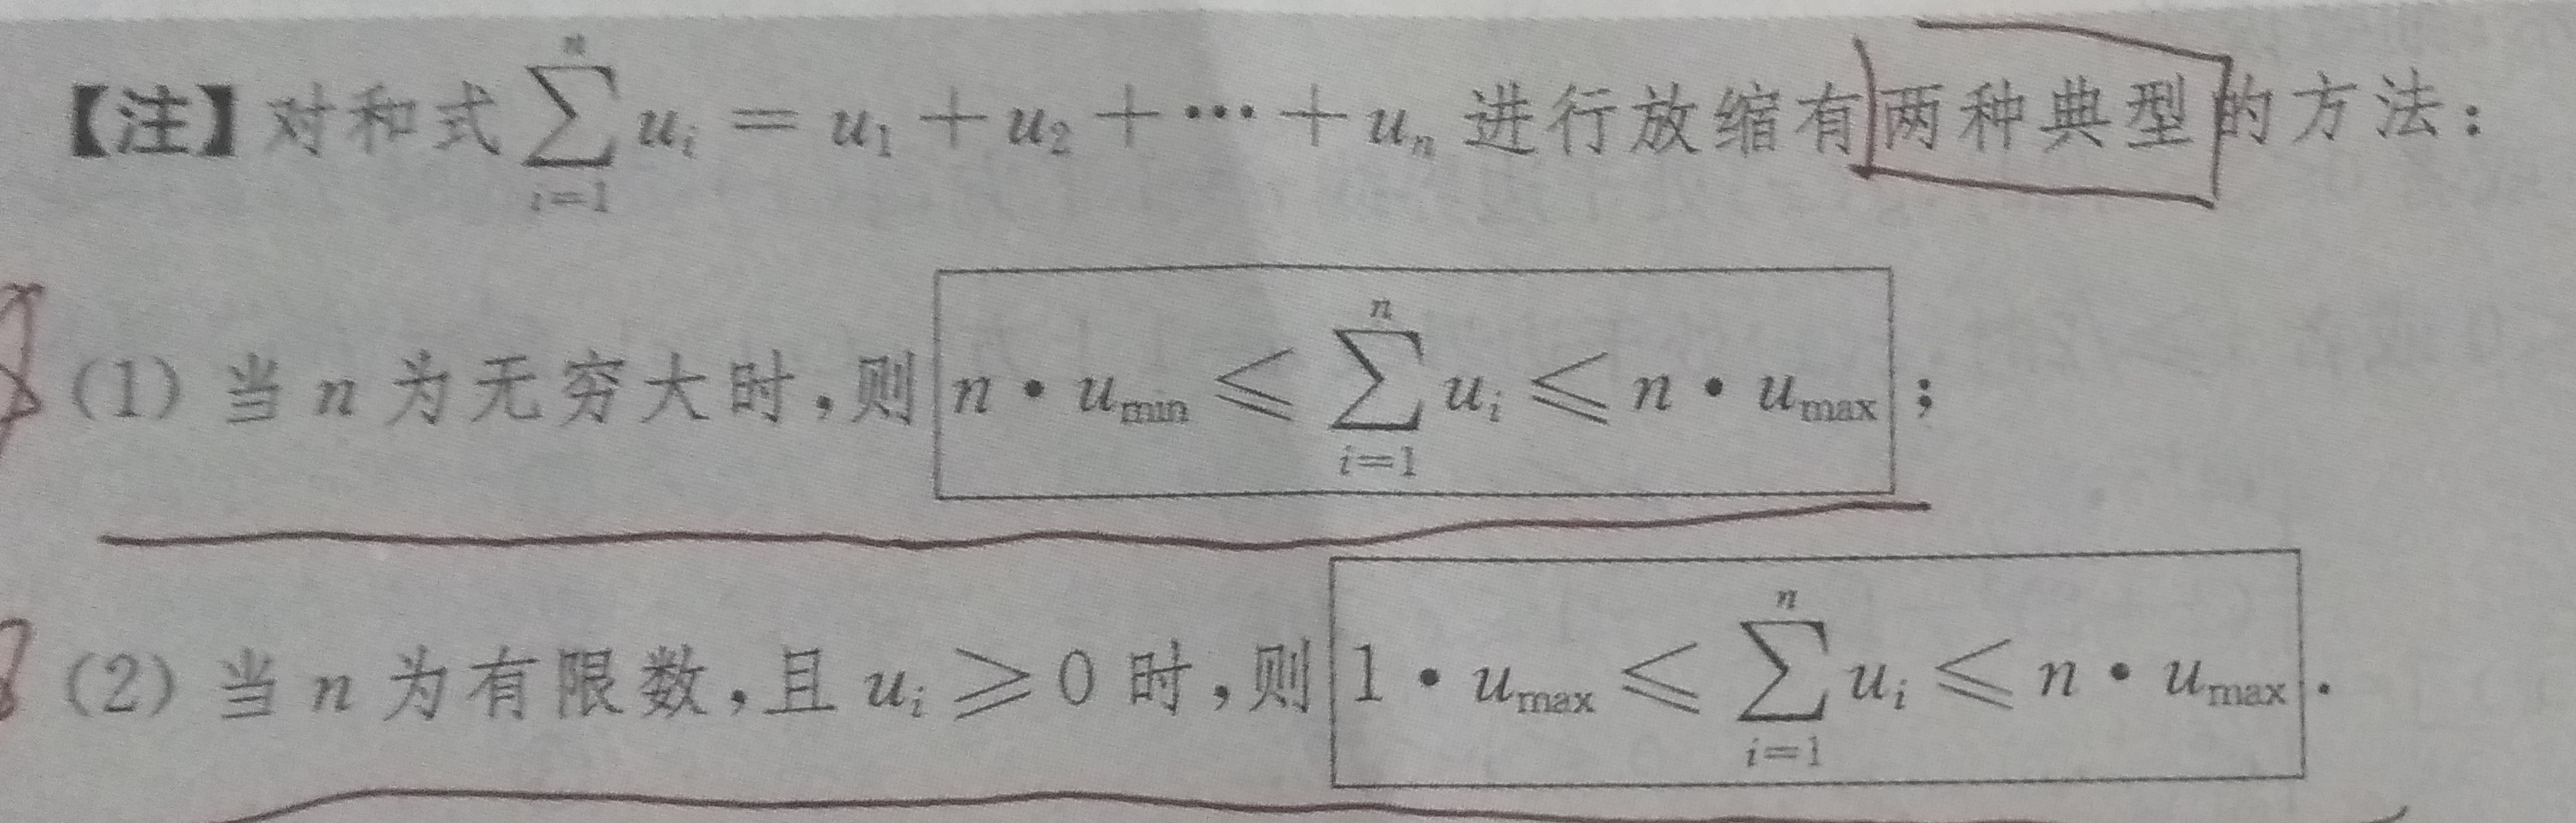
\includegraphics{9345E7/9345E74D588F5883C9985F64C9B1.jpg}
\item
  极限比较\\
  \[ f(x) \geq g(x) \rightarrow \lim f(x) \geq \lim g(x) \]
  \[ \lim f(x) > \lim g(x) \rightarrow f(x) > g(x) \]\\
  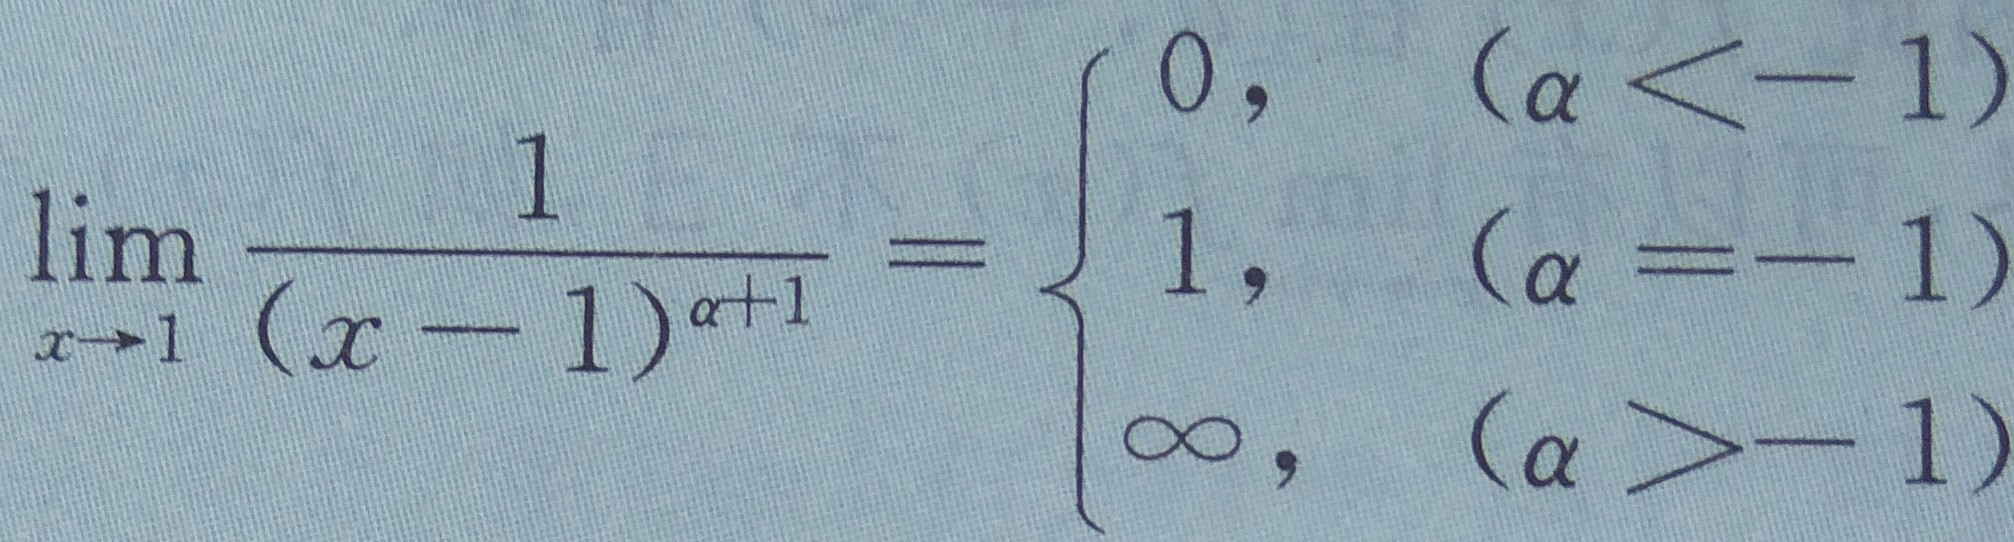
\includegraphics{9345E7/FA713494D7721783E05C994D3FC274D0.jpg}
  \[ [u(x)v(x)w(x)]'= u'(x)v(x)w(x)+u(x)v'(x)w(x)+u(x)v(x)w'(x)\]
  \[ \frac{\partial f}{\partial x} \equiv \frac{\partial f}{\partial y} \equiv 0\ \leftrightarrow df({x,y}) \equiv 0 \]
  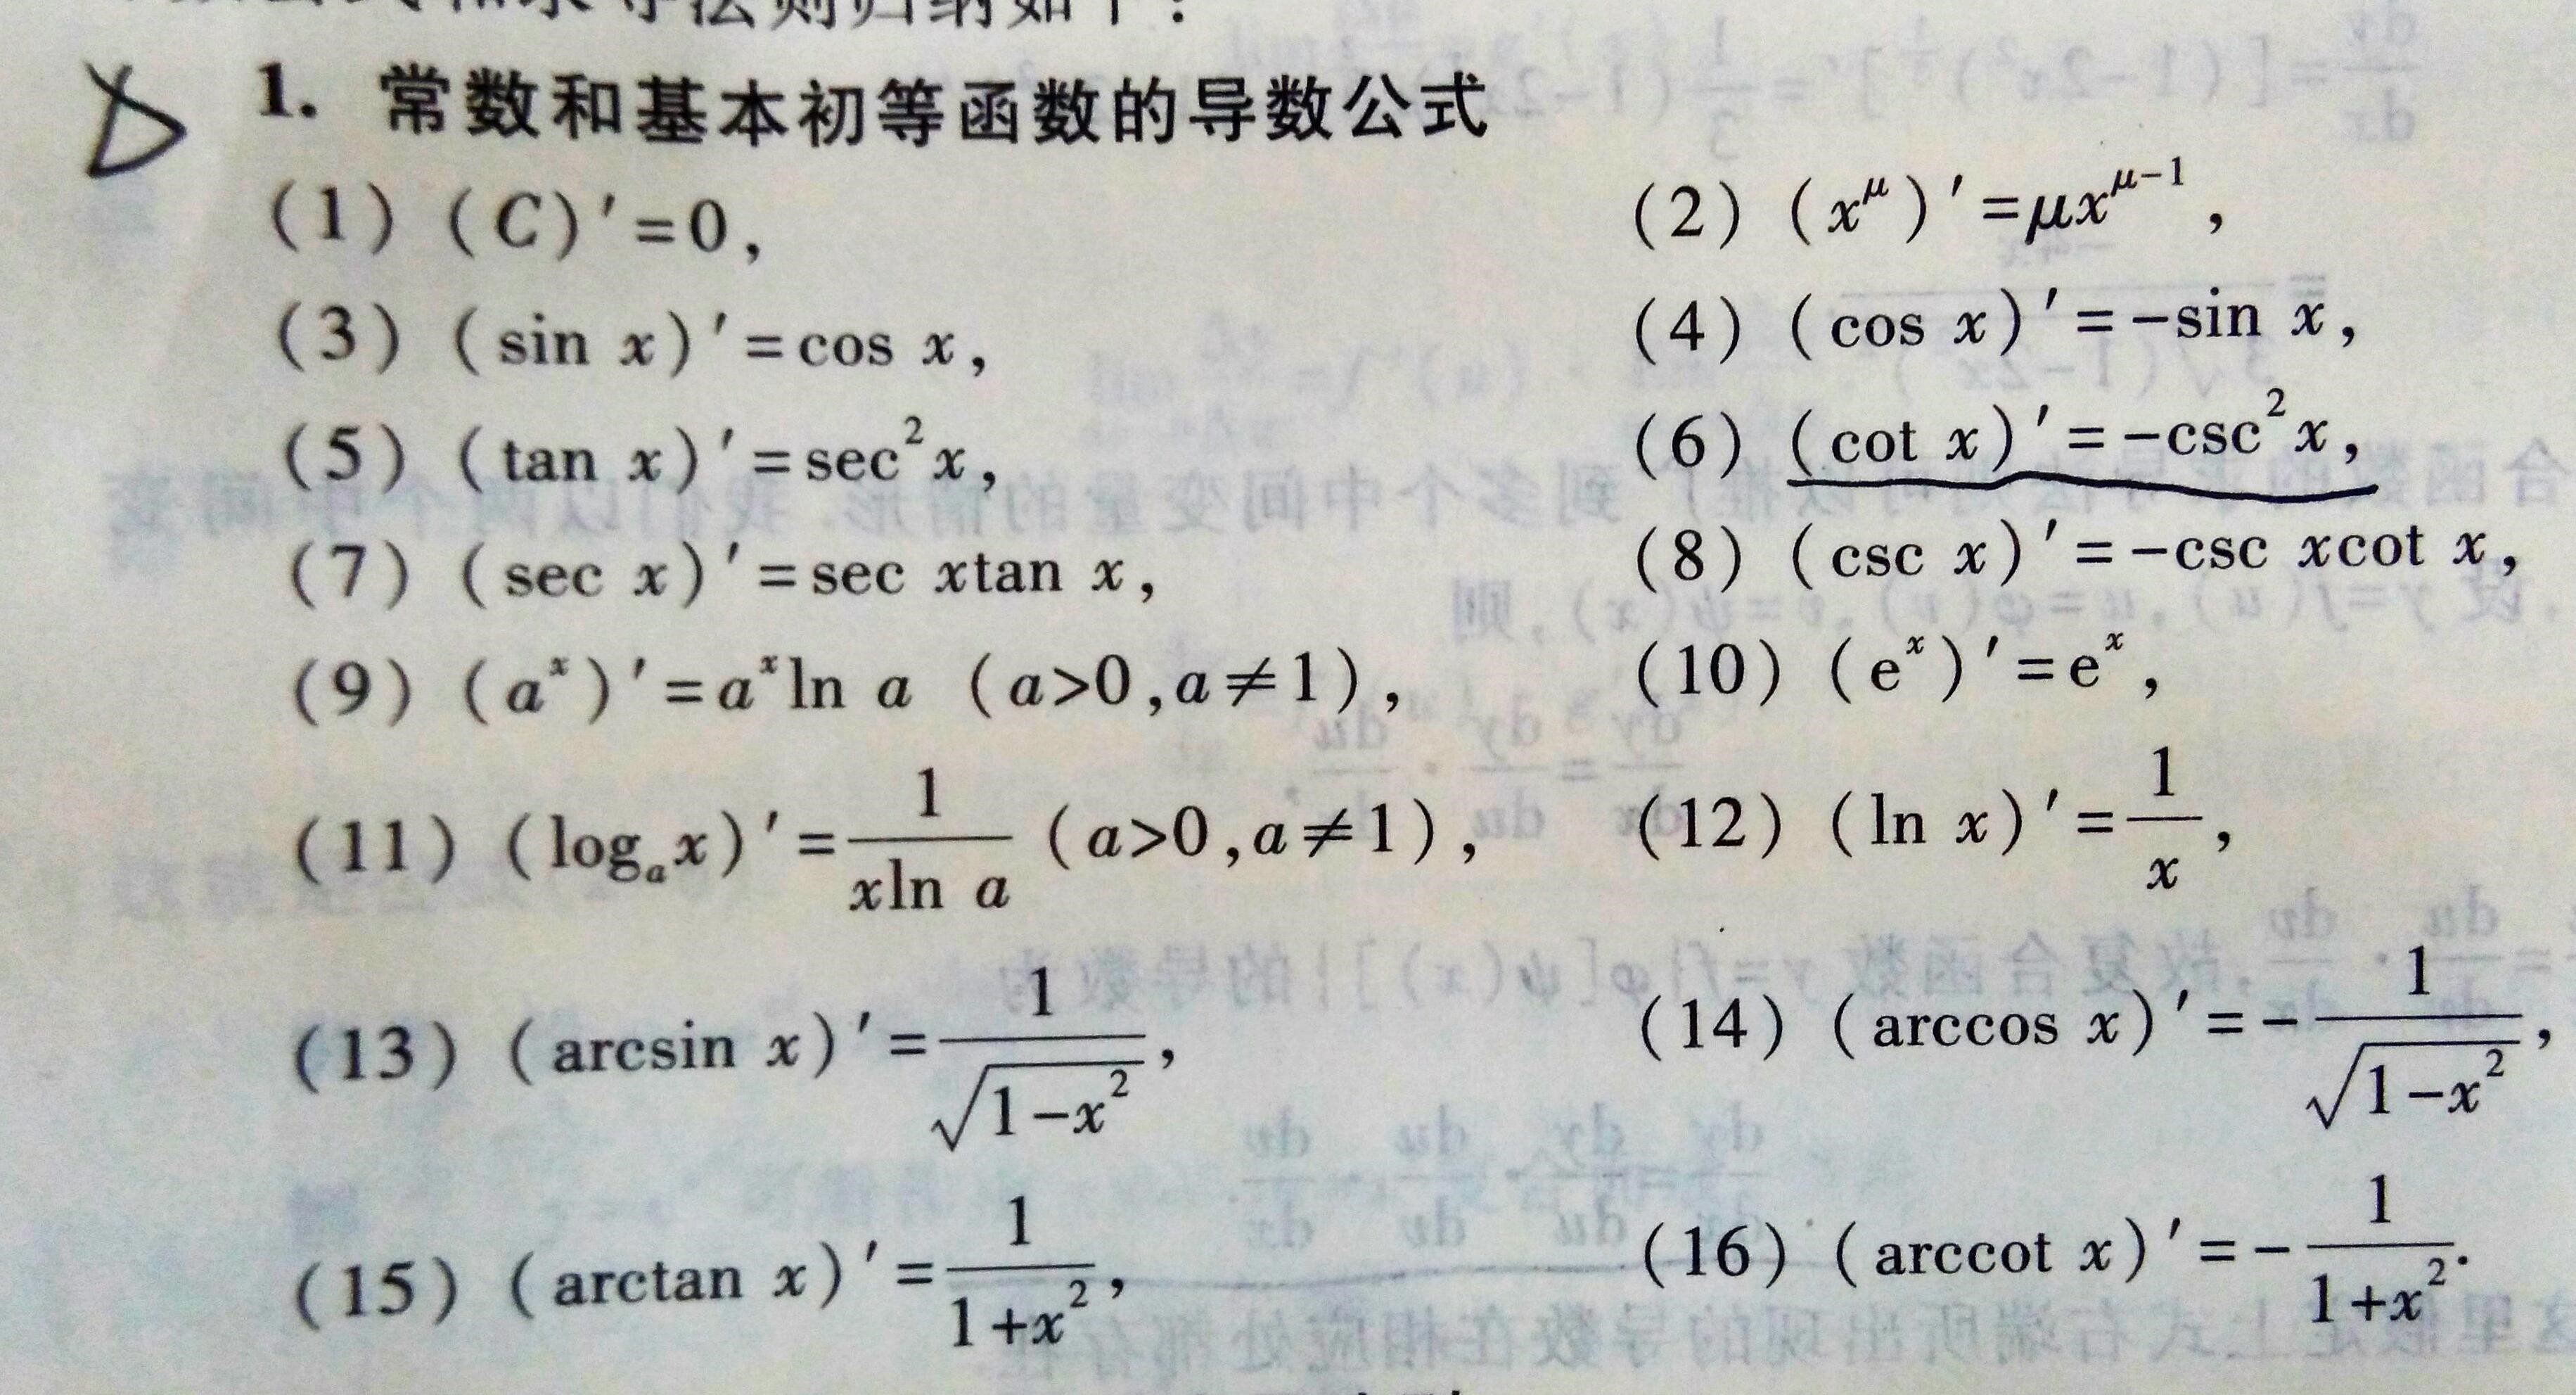
\includegraphics{9345E7/75F34B3DC01B176842127DE457F96A09.jpg}
\item
  球体积\\
  \[ V=\frac{4}{3} \pi R^3\]
\item
  表面积\\
  \[ S= 4 \pi R^2\]
\item
  定积分定义\\
  \[ \int_a^b f(x)dx= \lim_{n \rightarrow \infty } \sum_{i=1}^n \frac{f \left( a+ \frac{b-a}{n}i \right)(b-a)}{n}\]\\
\item
  连续函数必有原函数\\
  1.1. 含有第一类间断点,无穷间断点的函数在包含间断点的区间没有原函数\\
  1.1. 跳跃间断点可以有原函数
\item
  基本积分表
  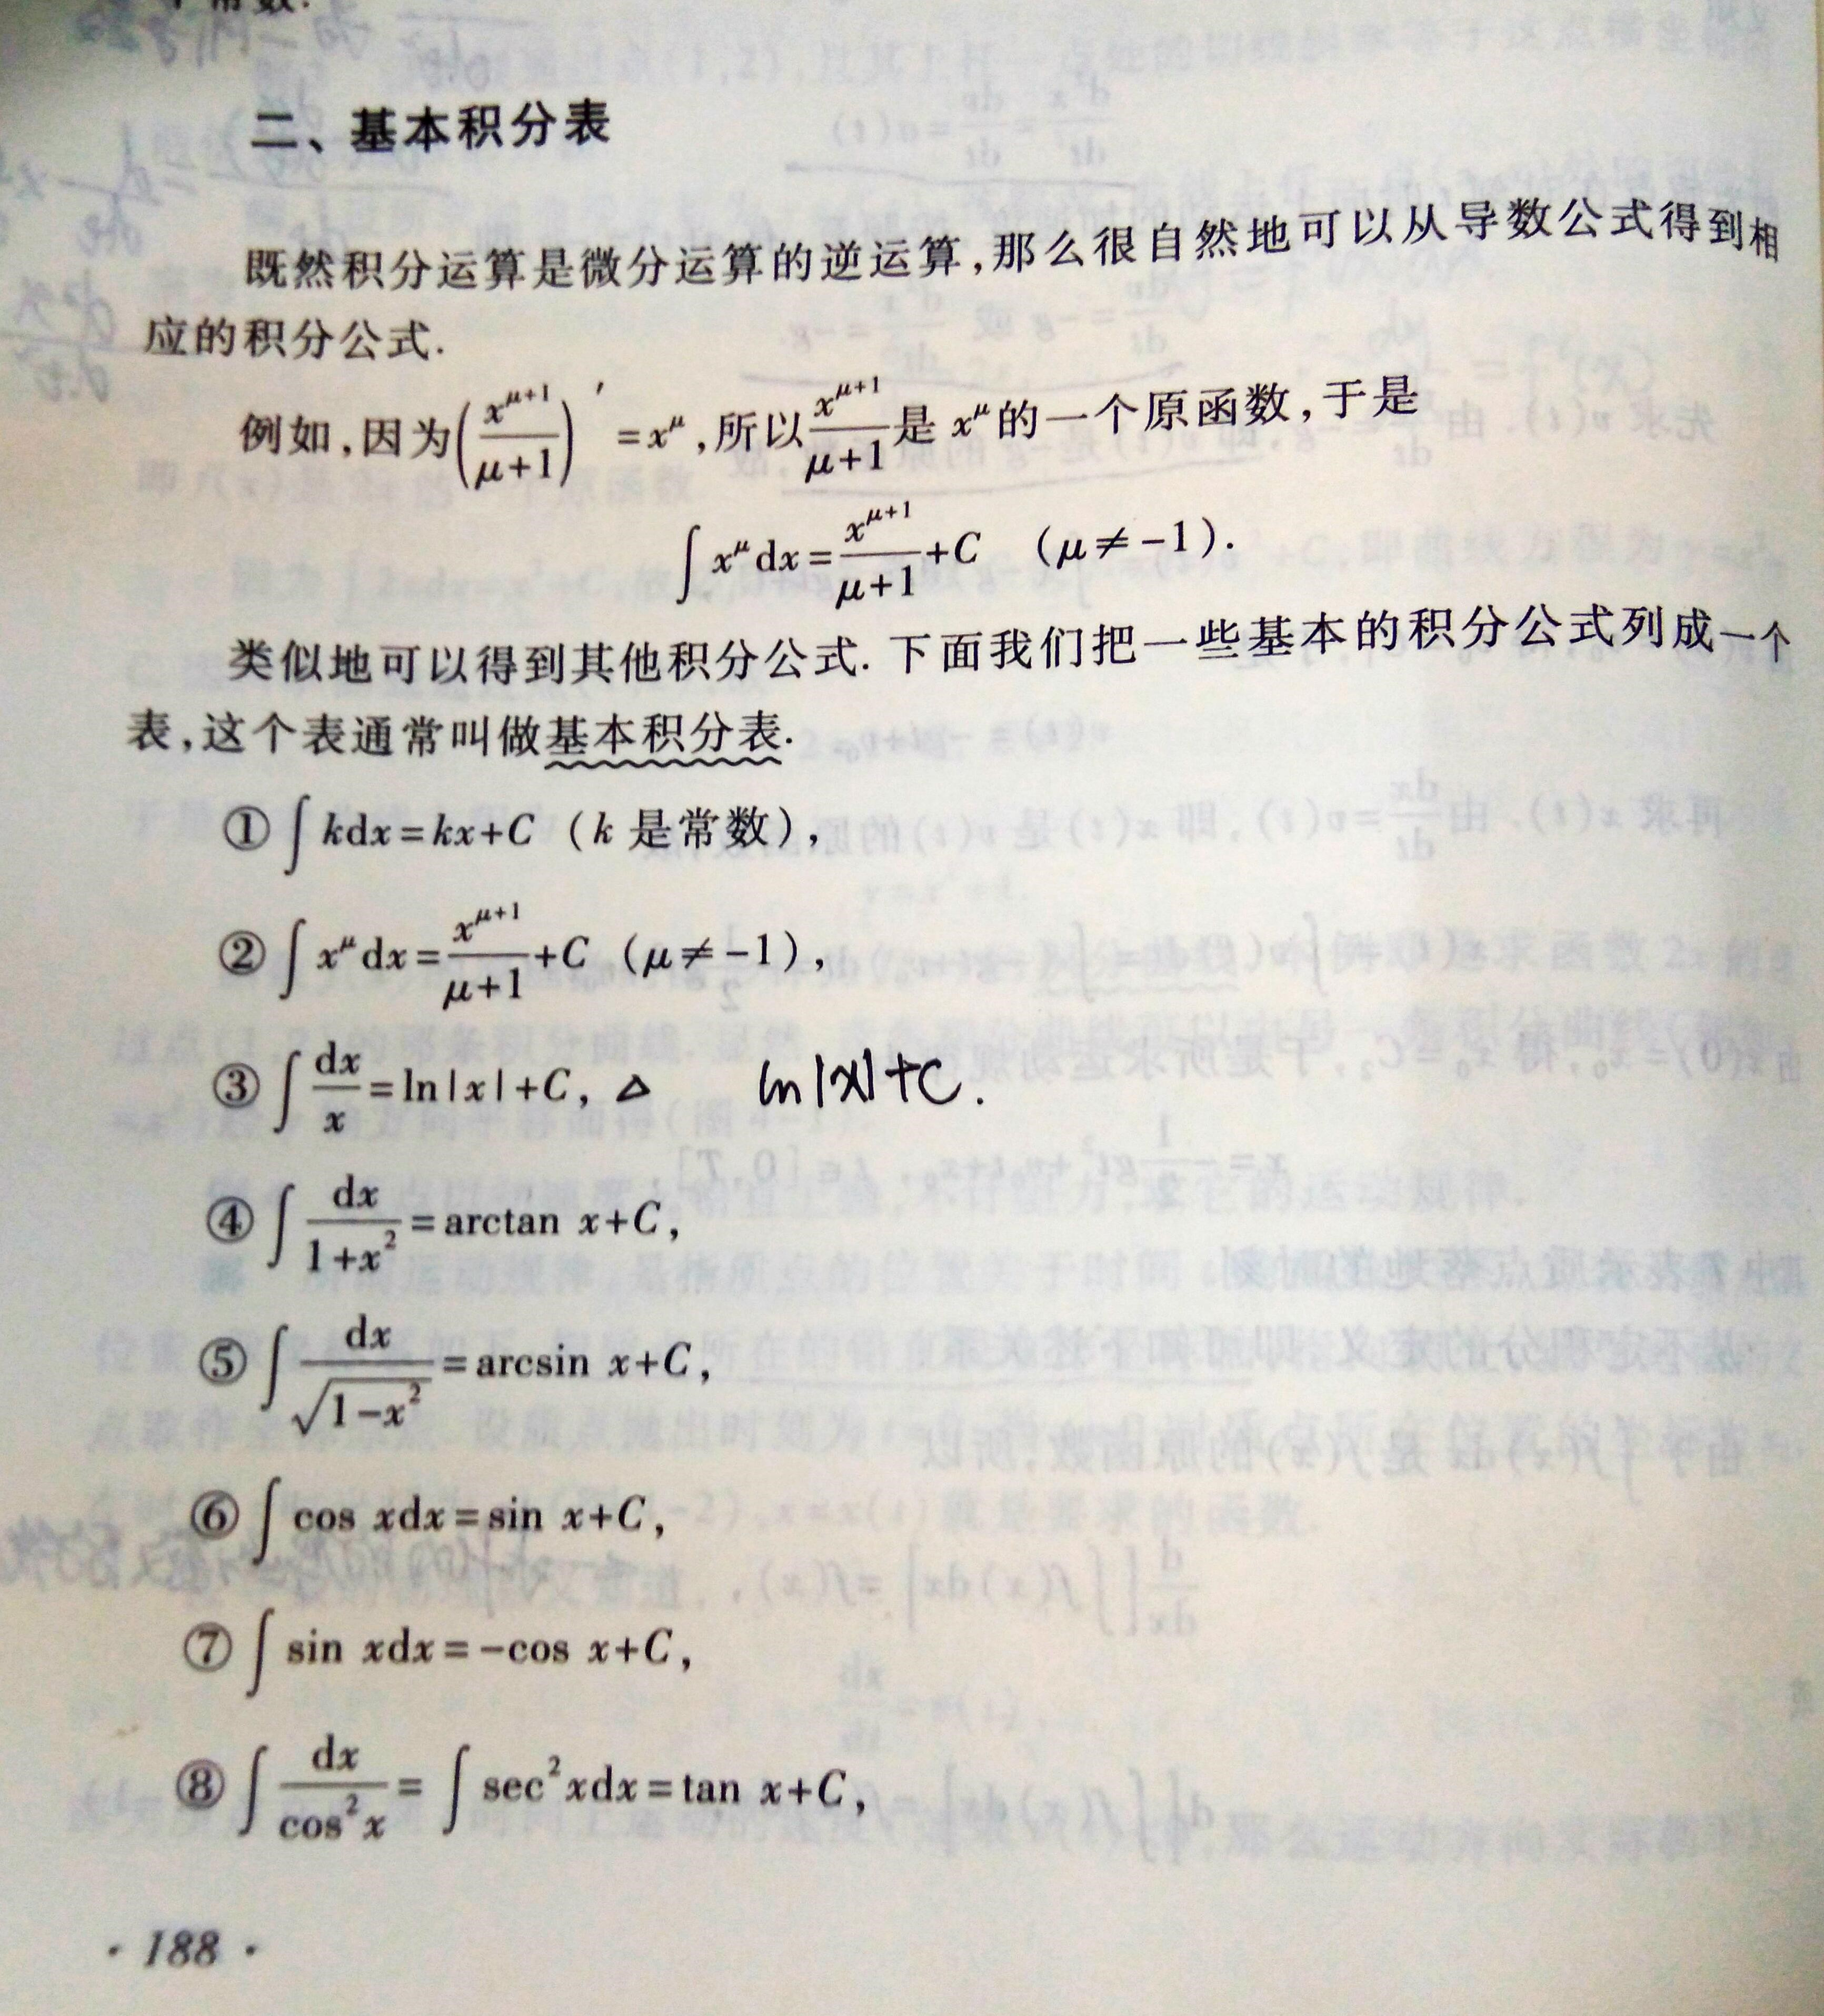
\includegraphics{9345E7/9476215E0863B8FB681EC9D2BB921BDB.jpg}
  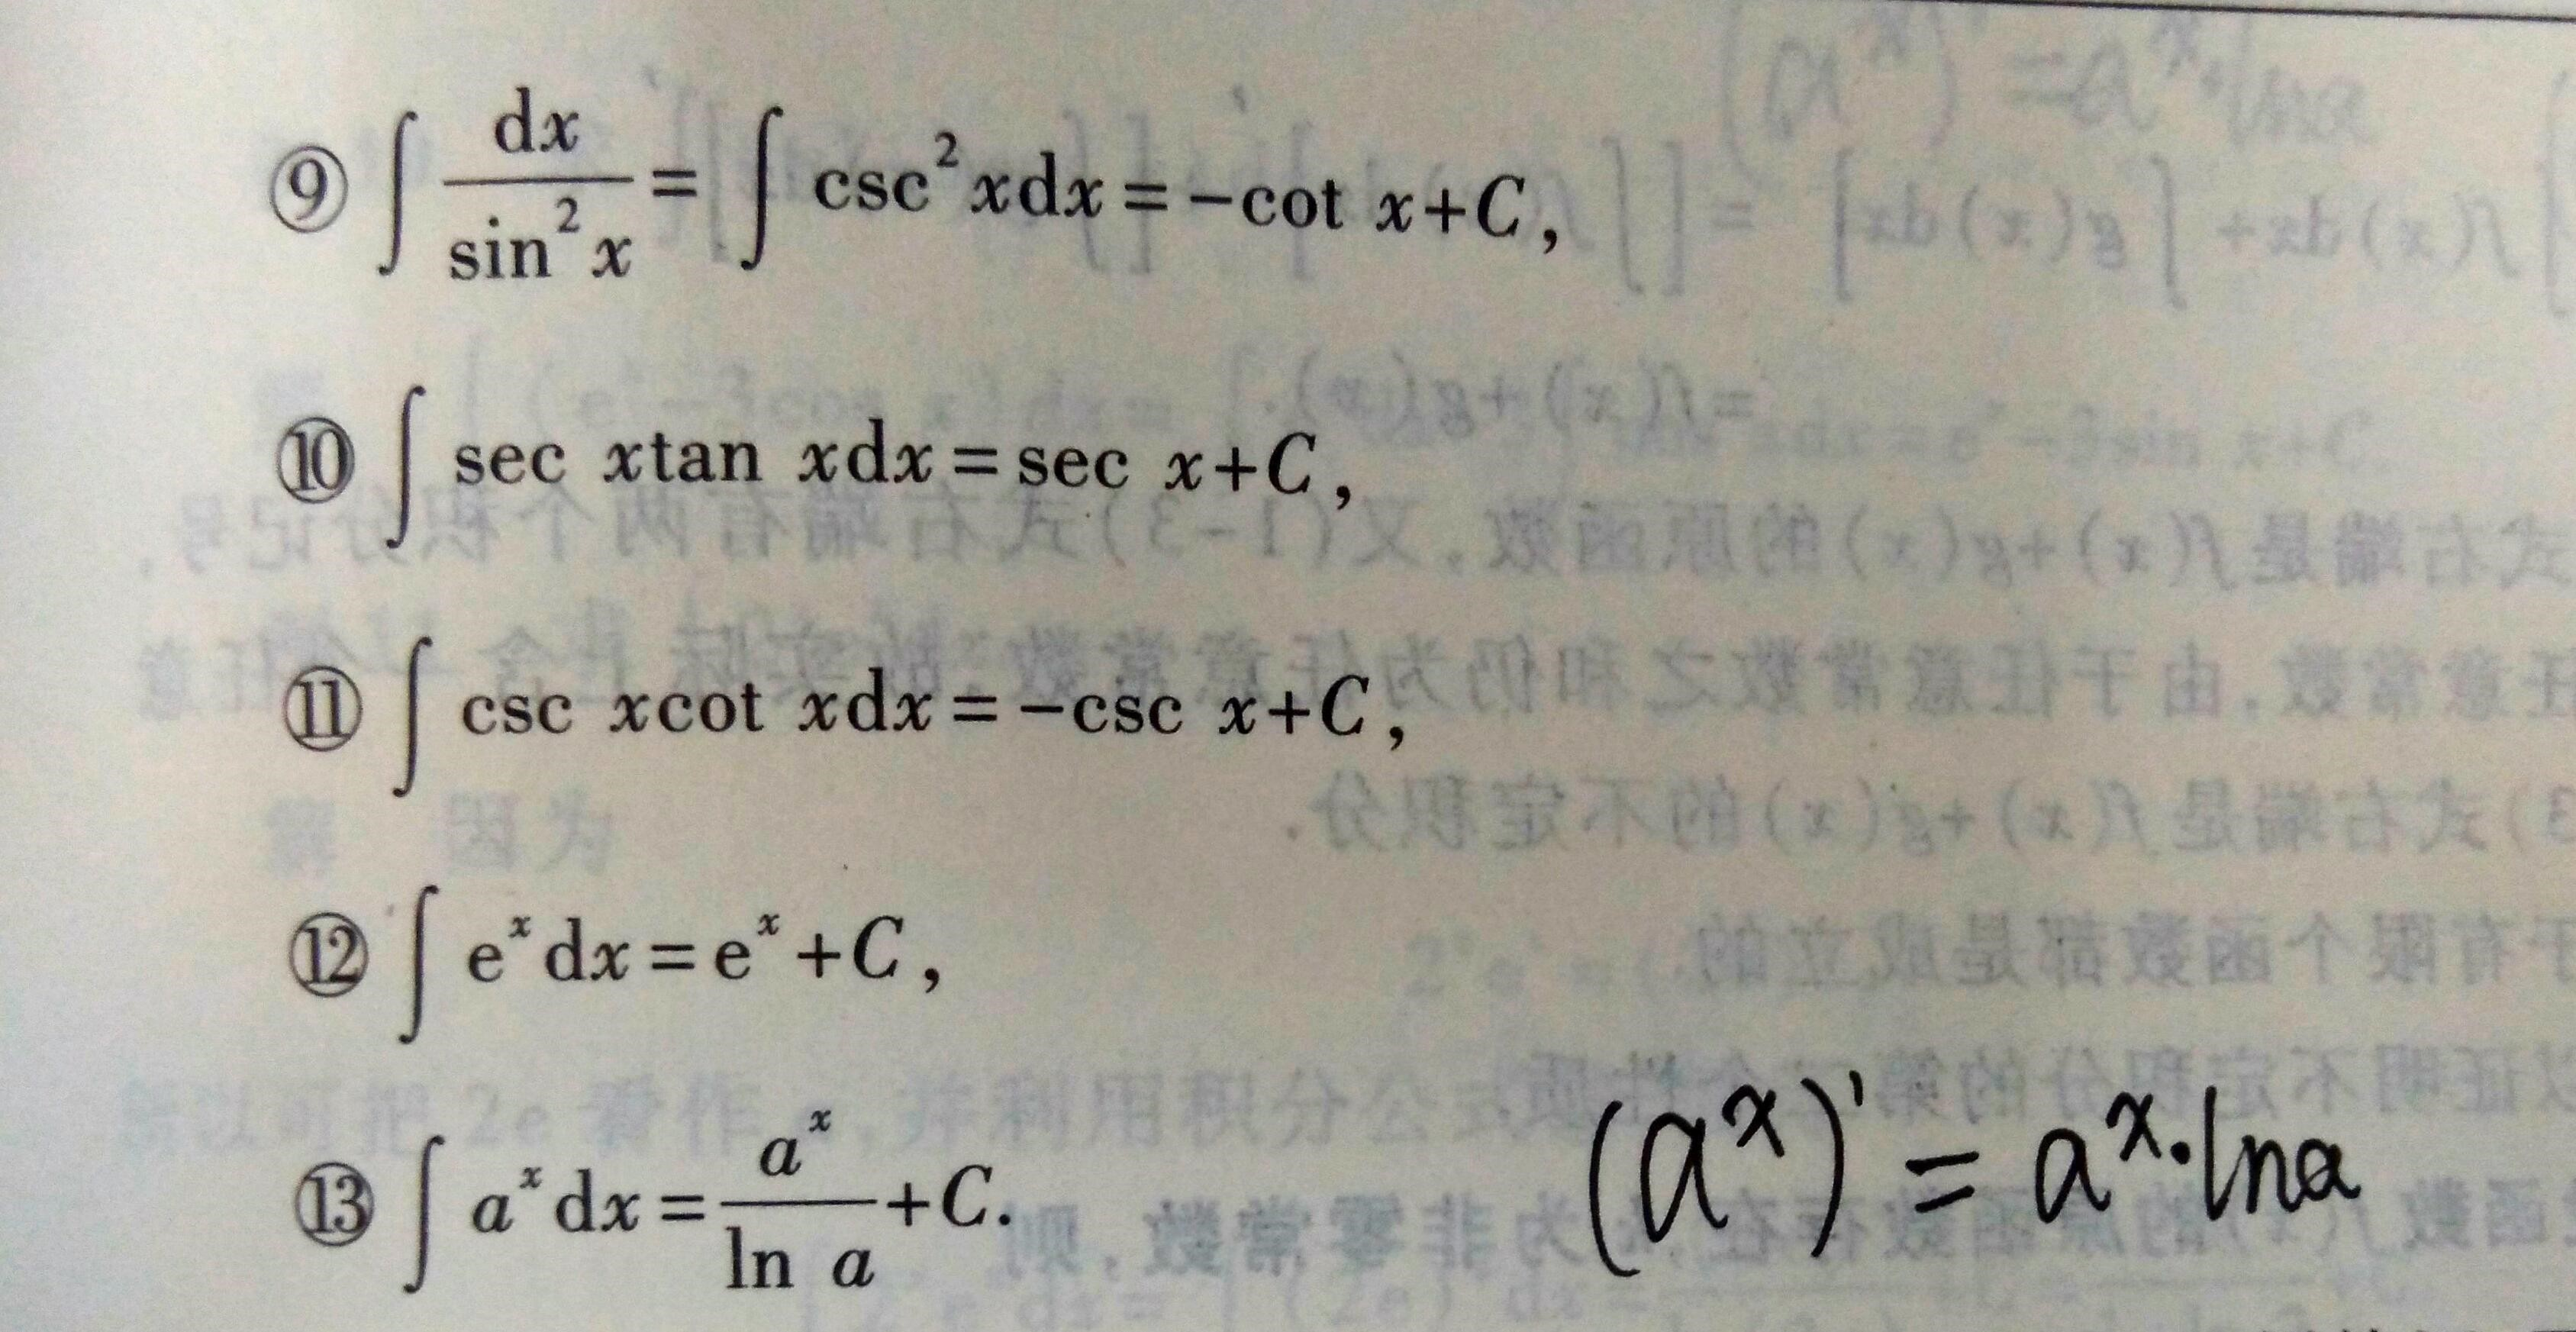
\includegraphics{9345E7/4FEE9C843E57935F87D1E16F255FA43E.jpg}
  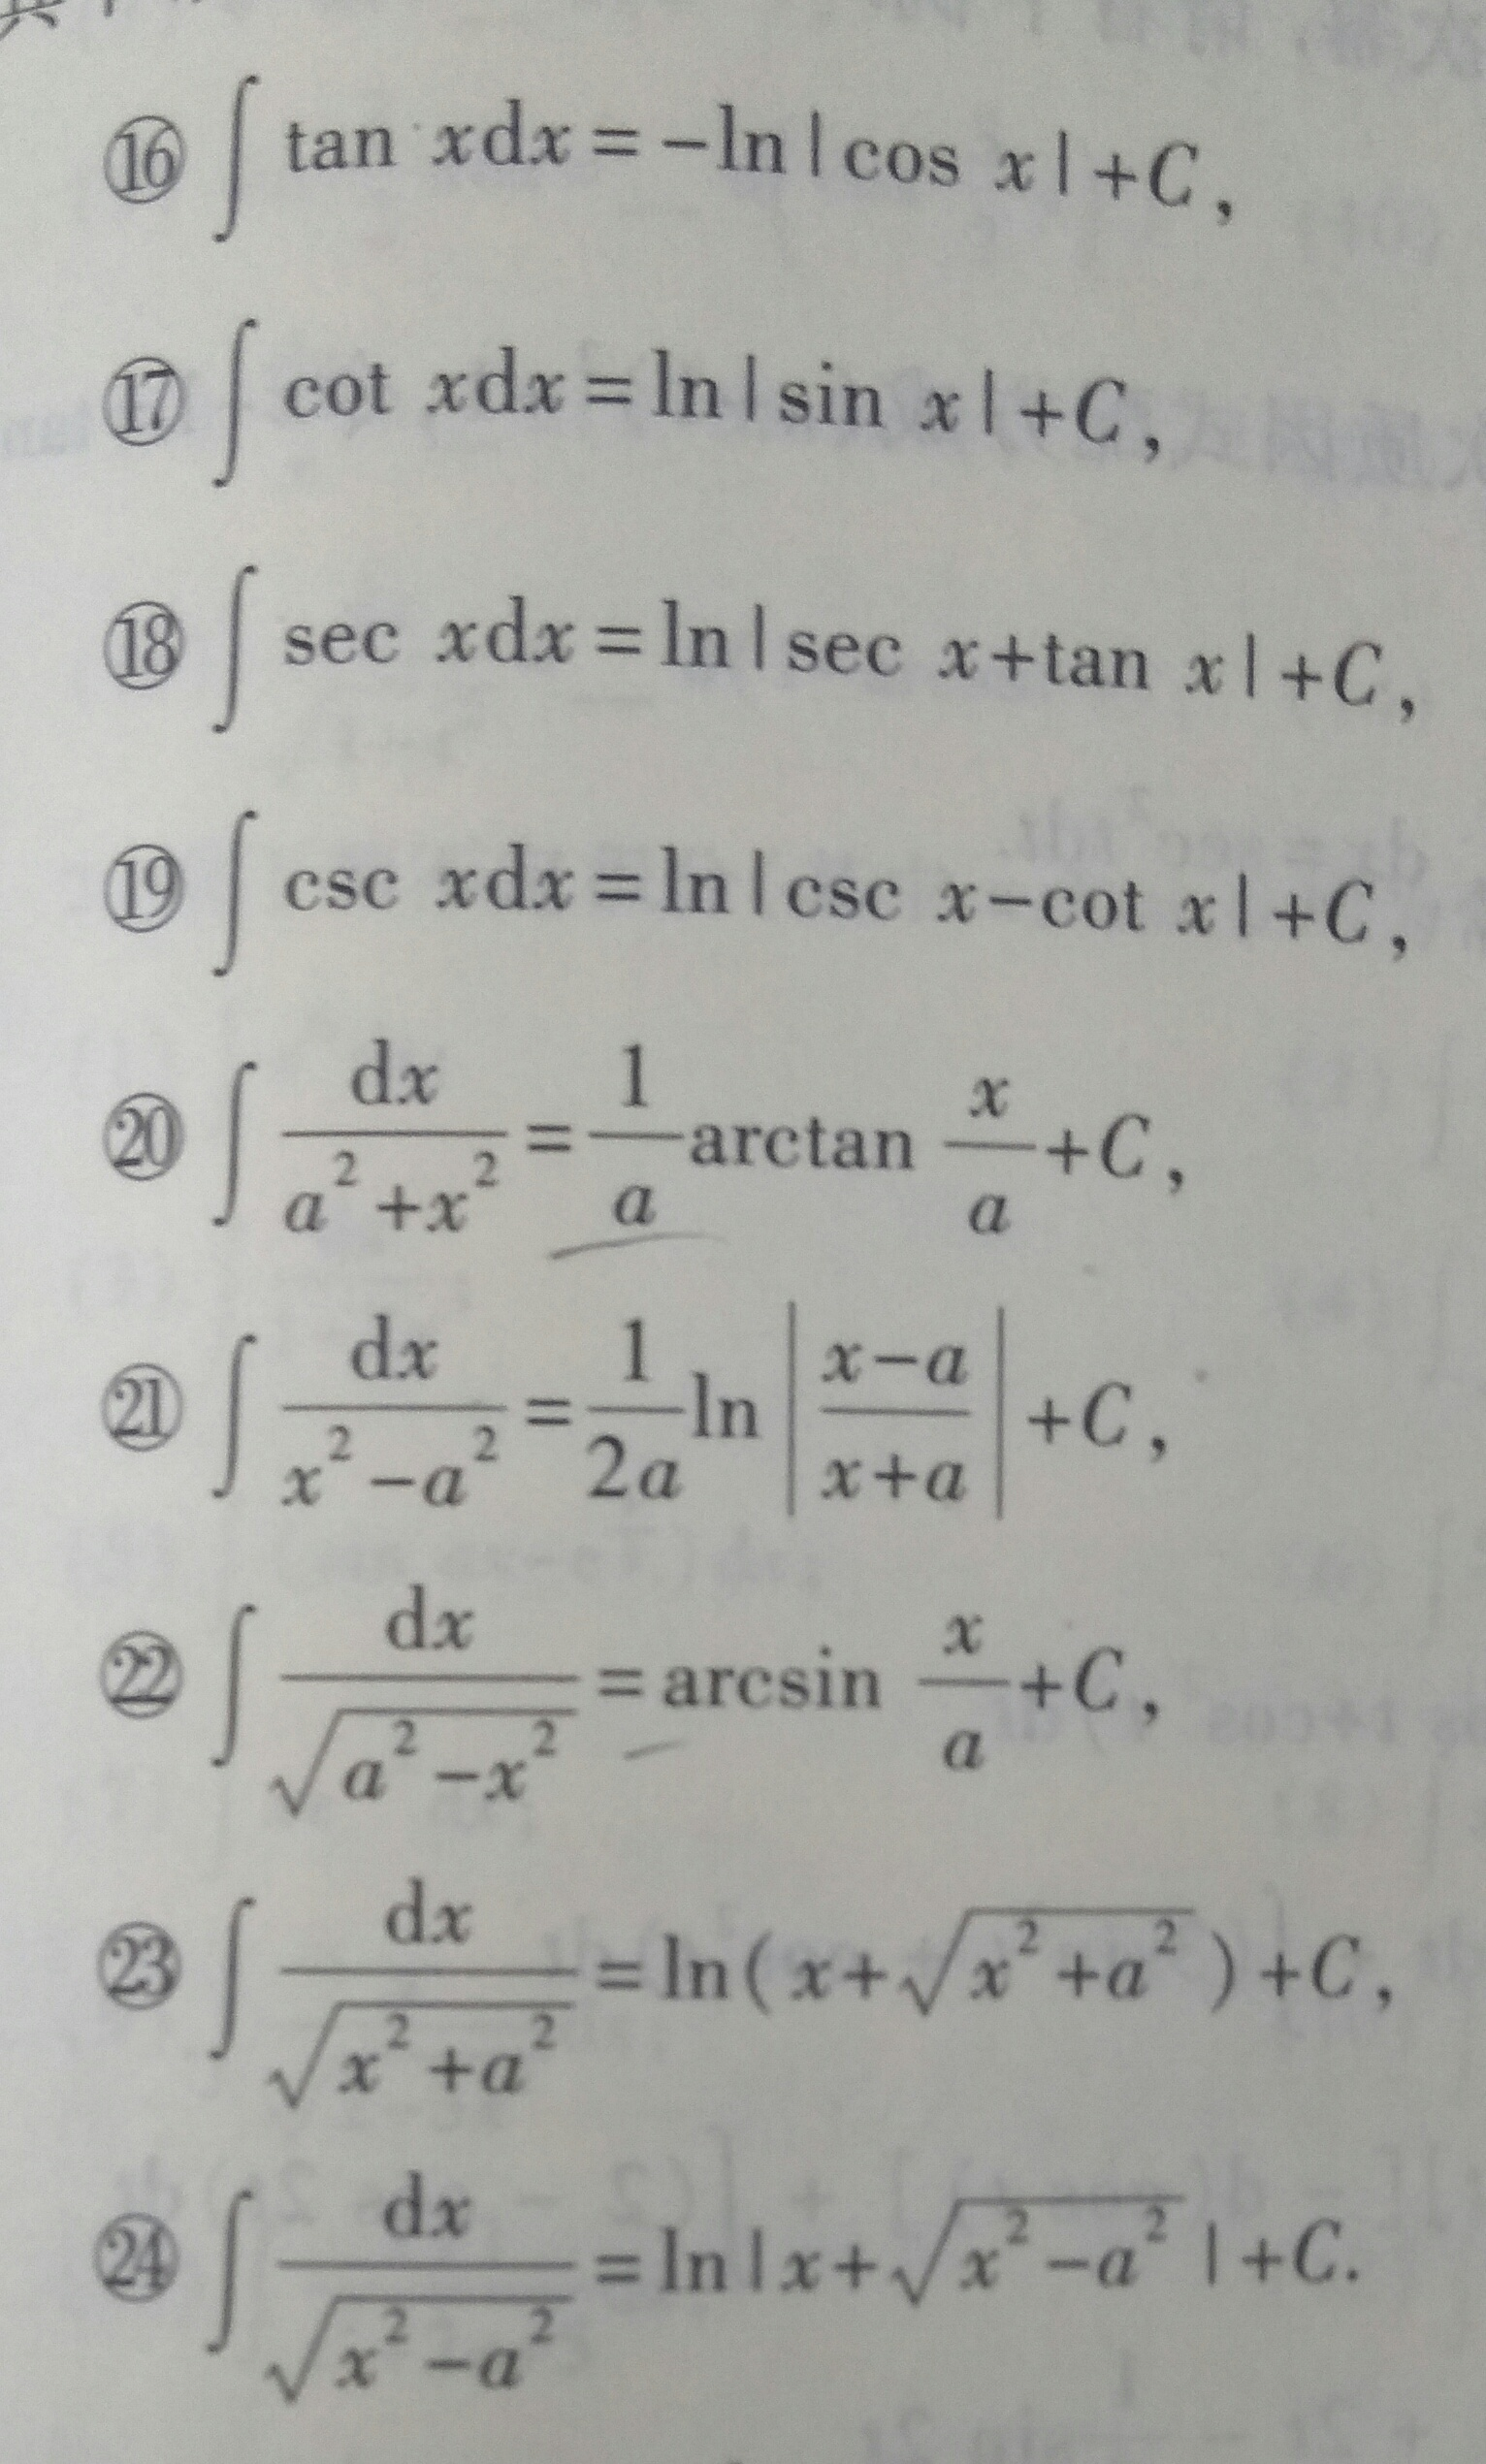
\includegraphics{9345E7/D70CA37458BBD6E13C00ADA8D5740222.jpg}
\item
  泰勒公式\\
  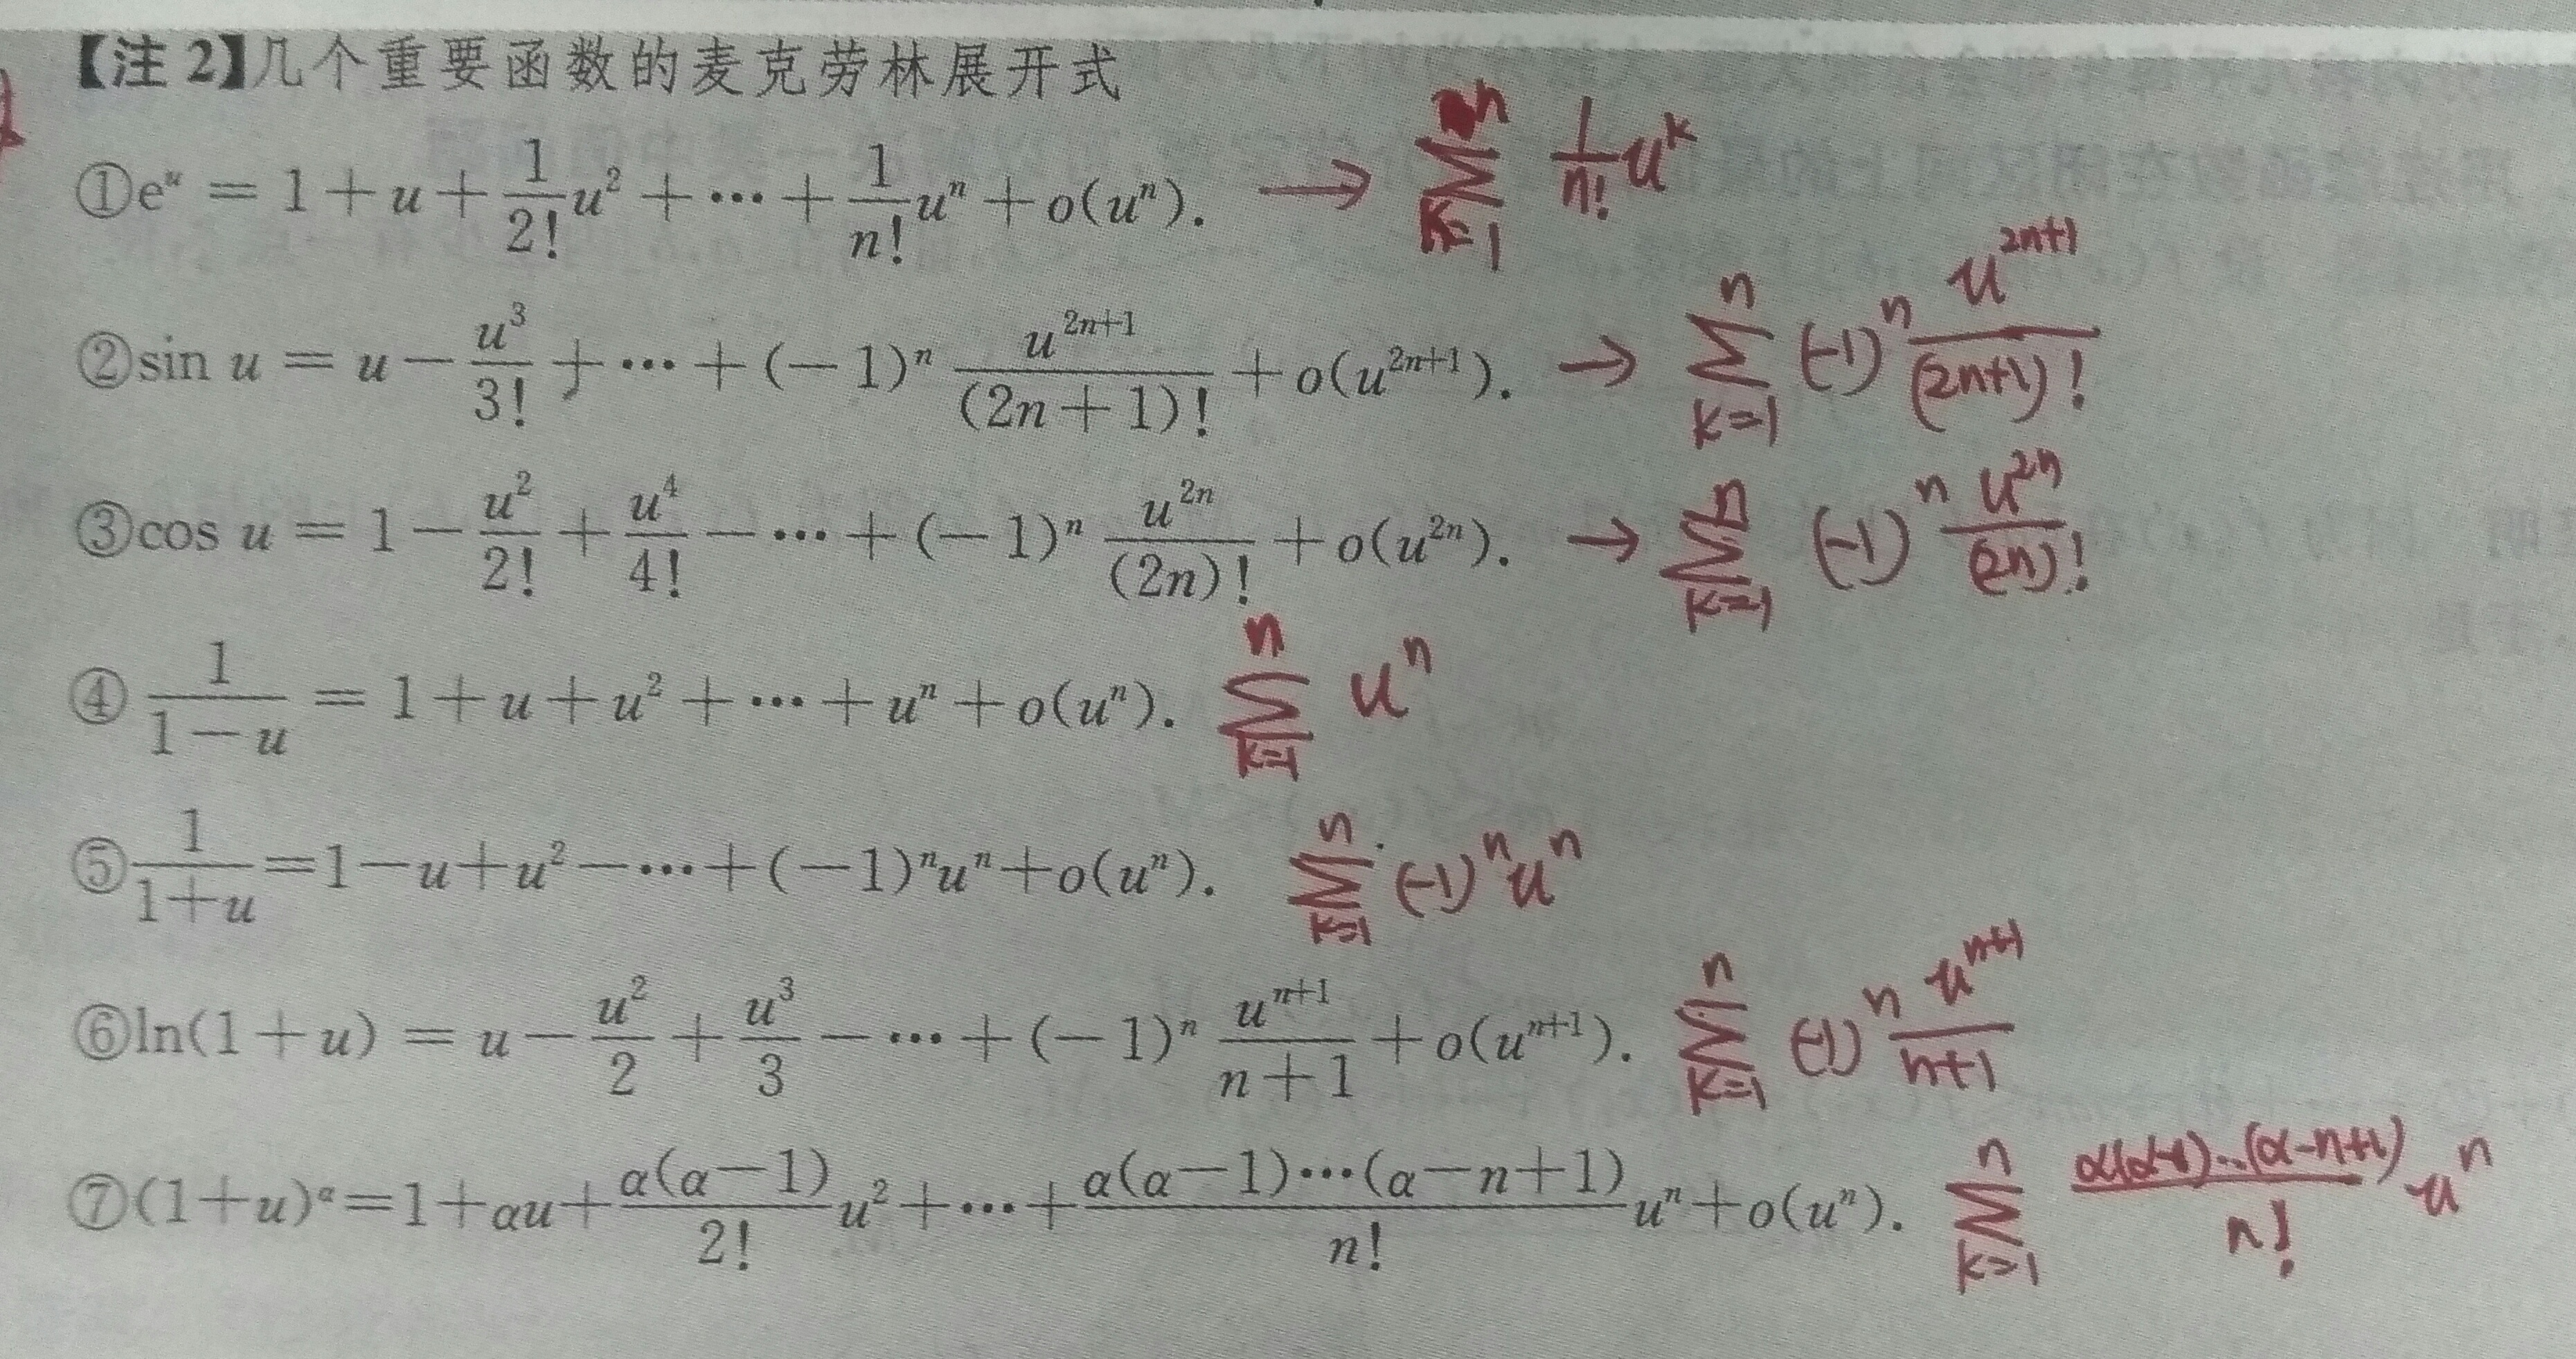
\includegraphics{9345E7/F04F85A8EB6EABFF18D6BE71383F2472.jpg}
  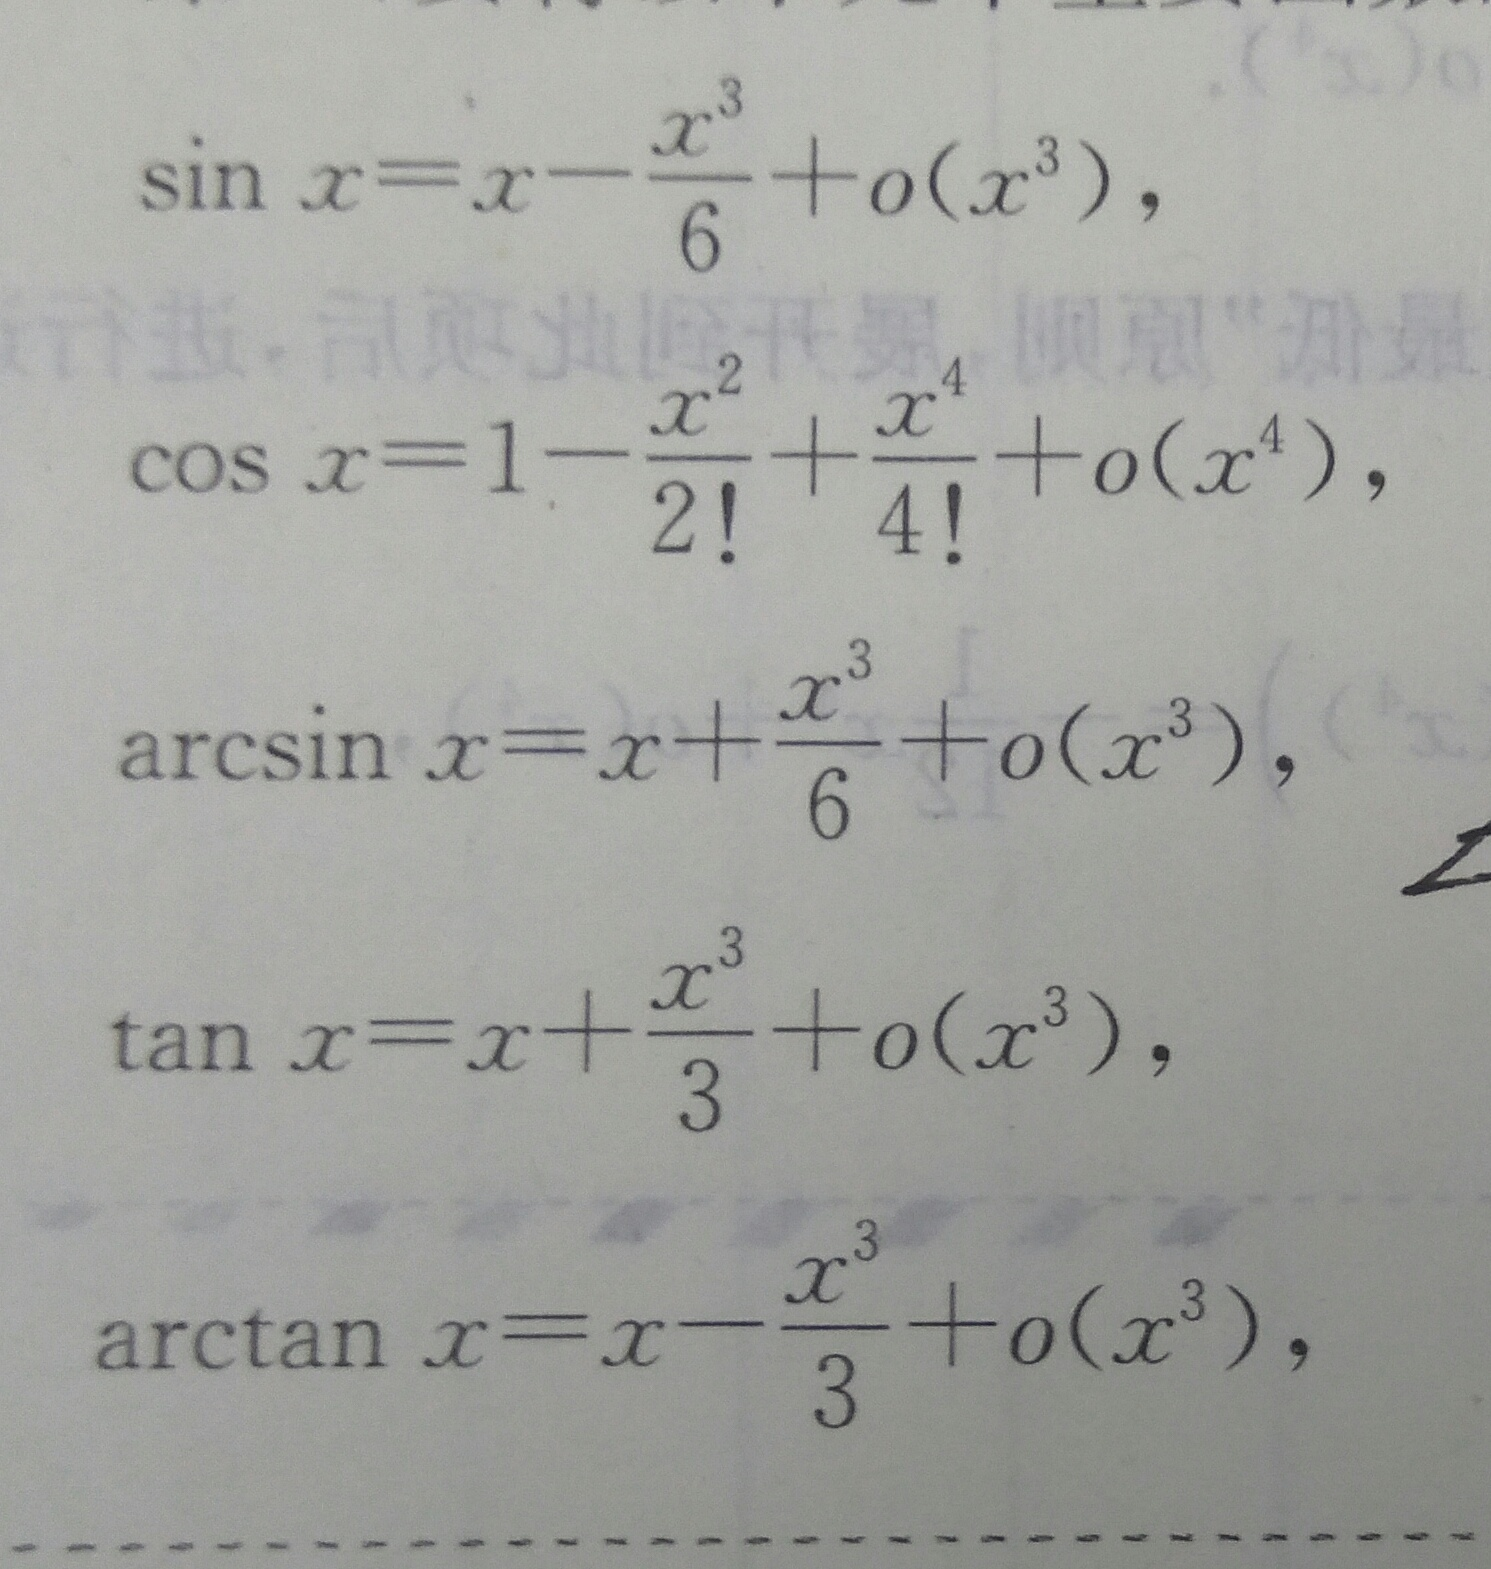
\includegraphics{9345E7/DBC6F35DE00EFED64F77BDBF8DE279EE.jpg}
\item
  几个初等函数的n阶导数公式\\
  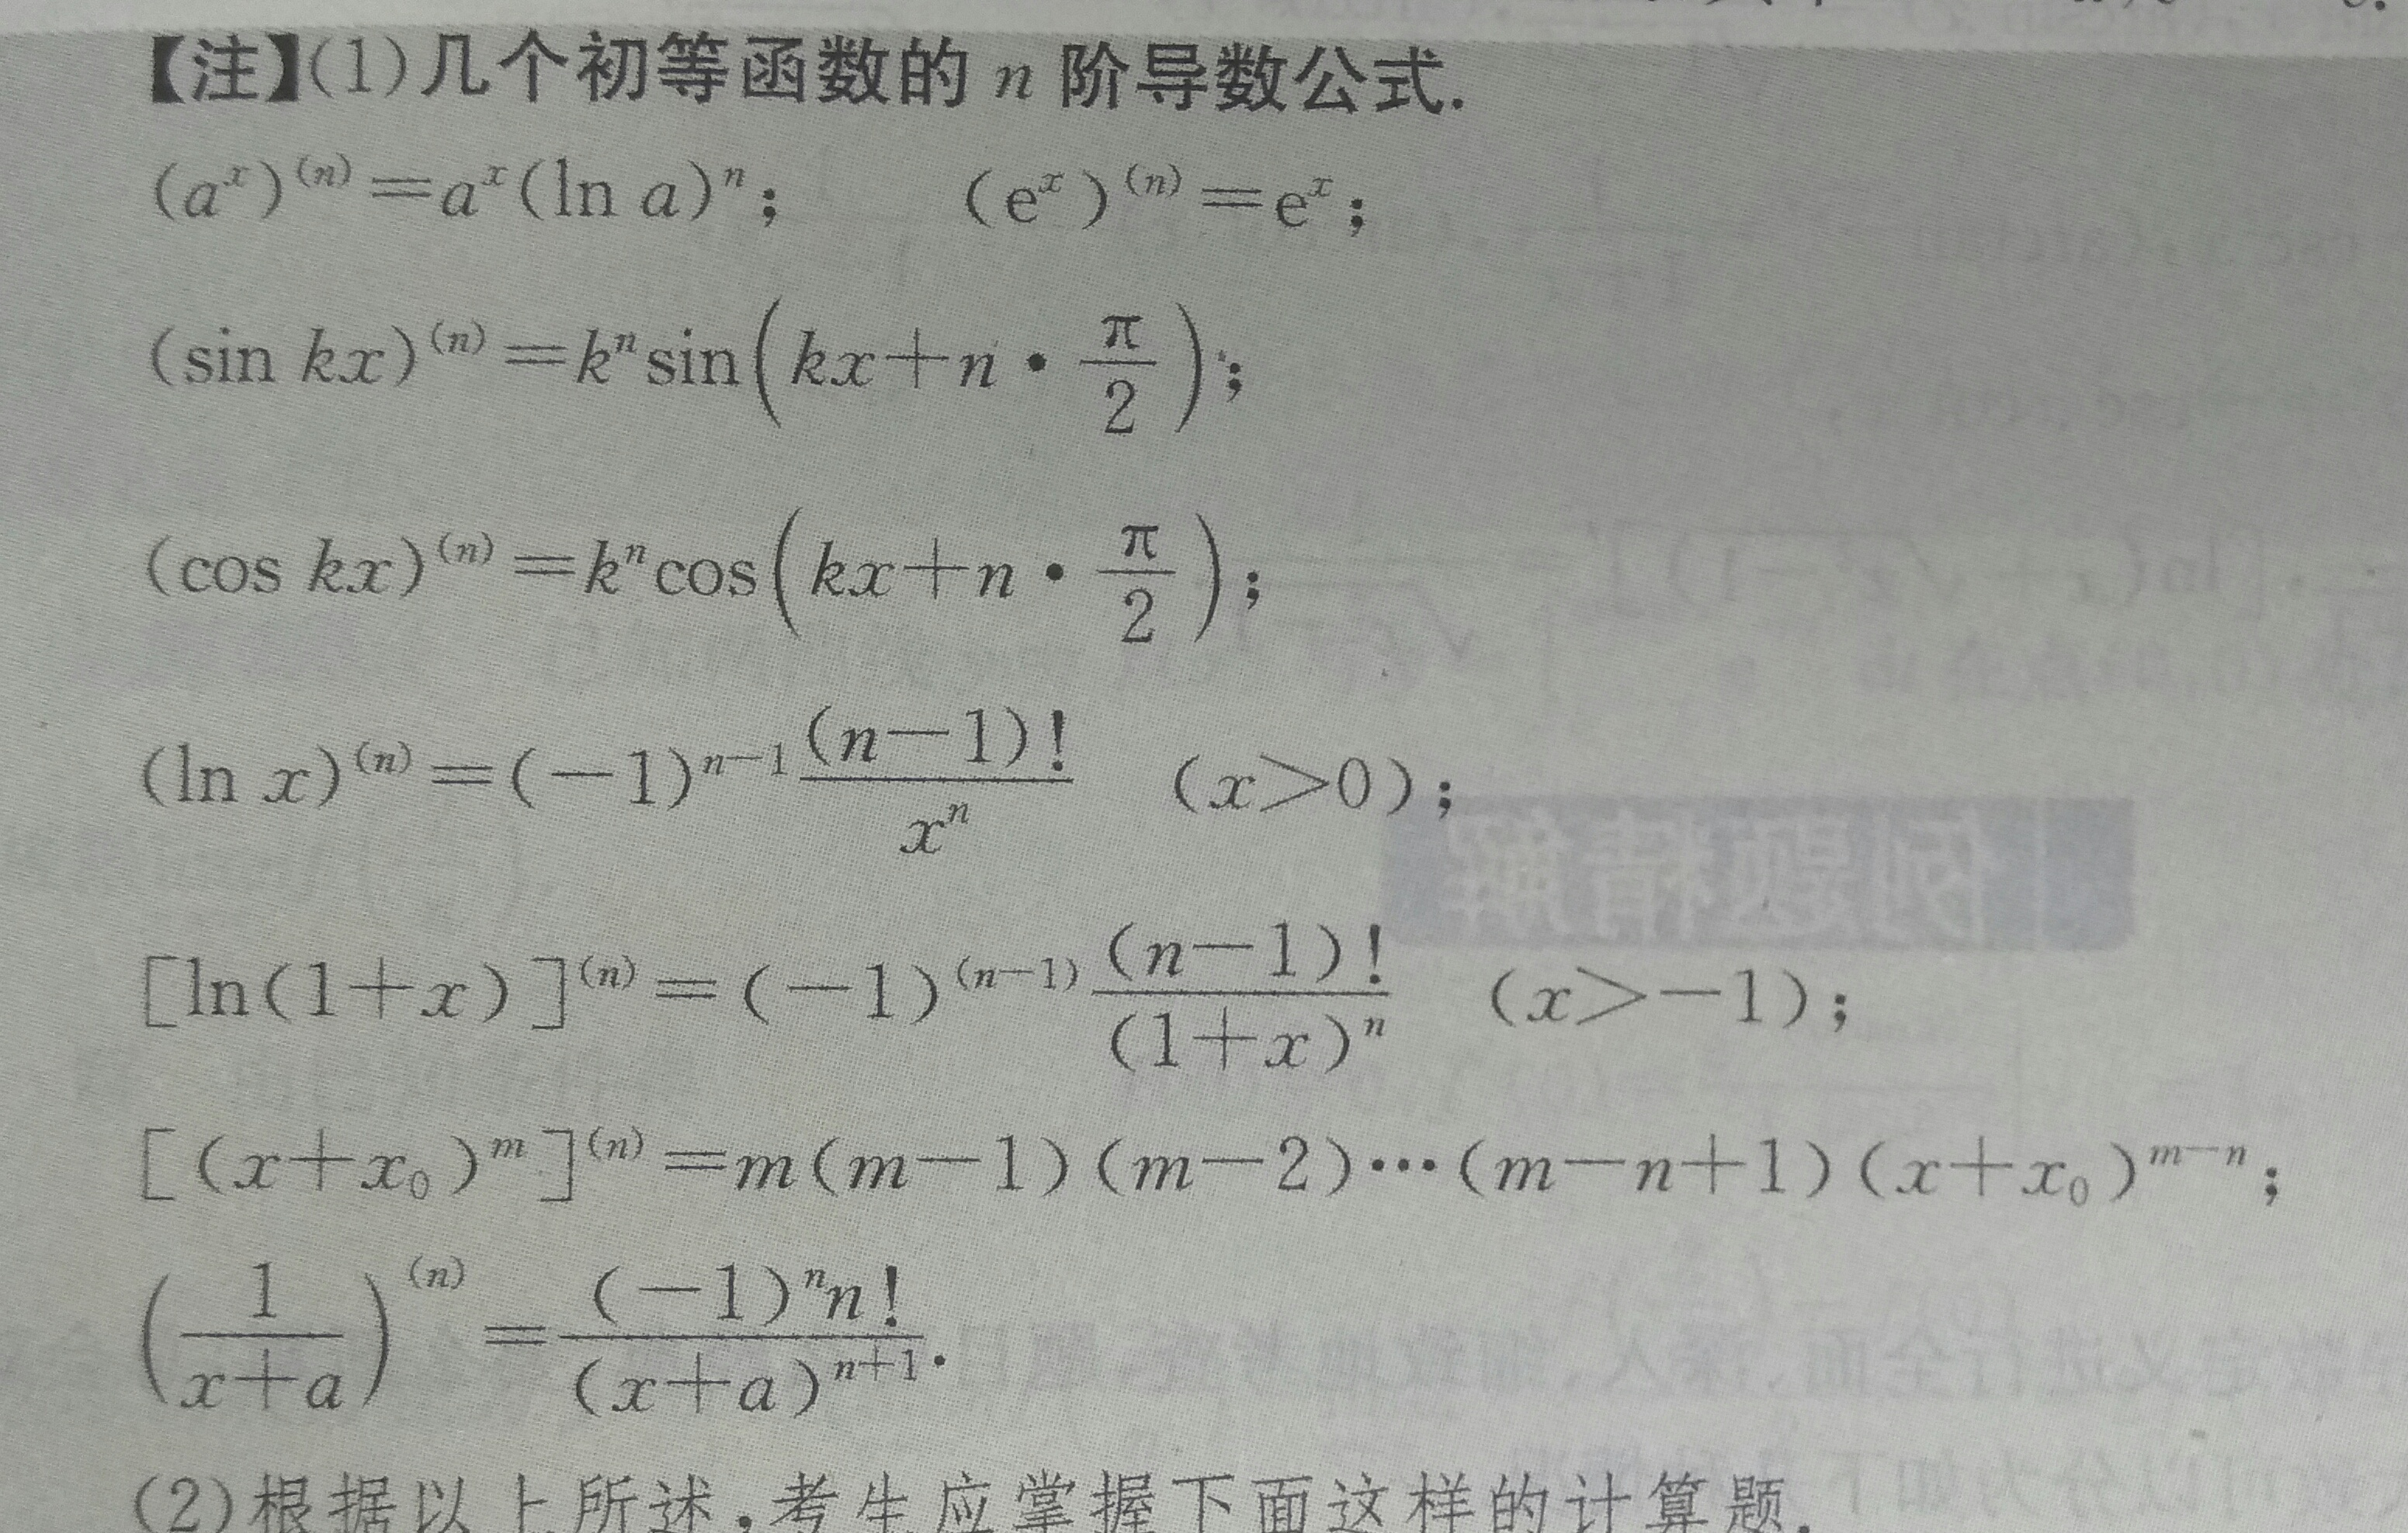
\includegraphics{9345E7/2A793F093B002F668B144F9ED087EB77.jpg}
  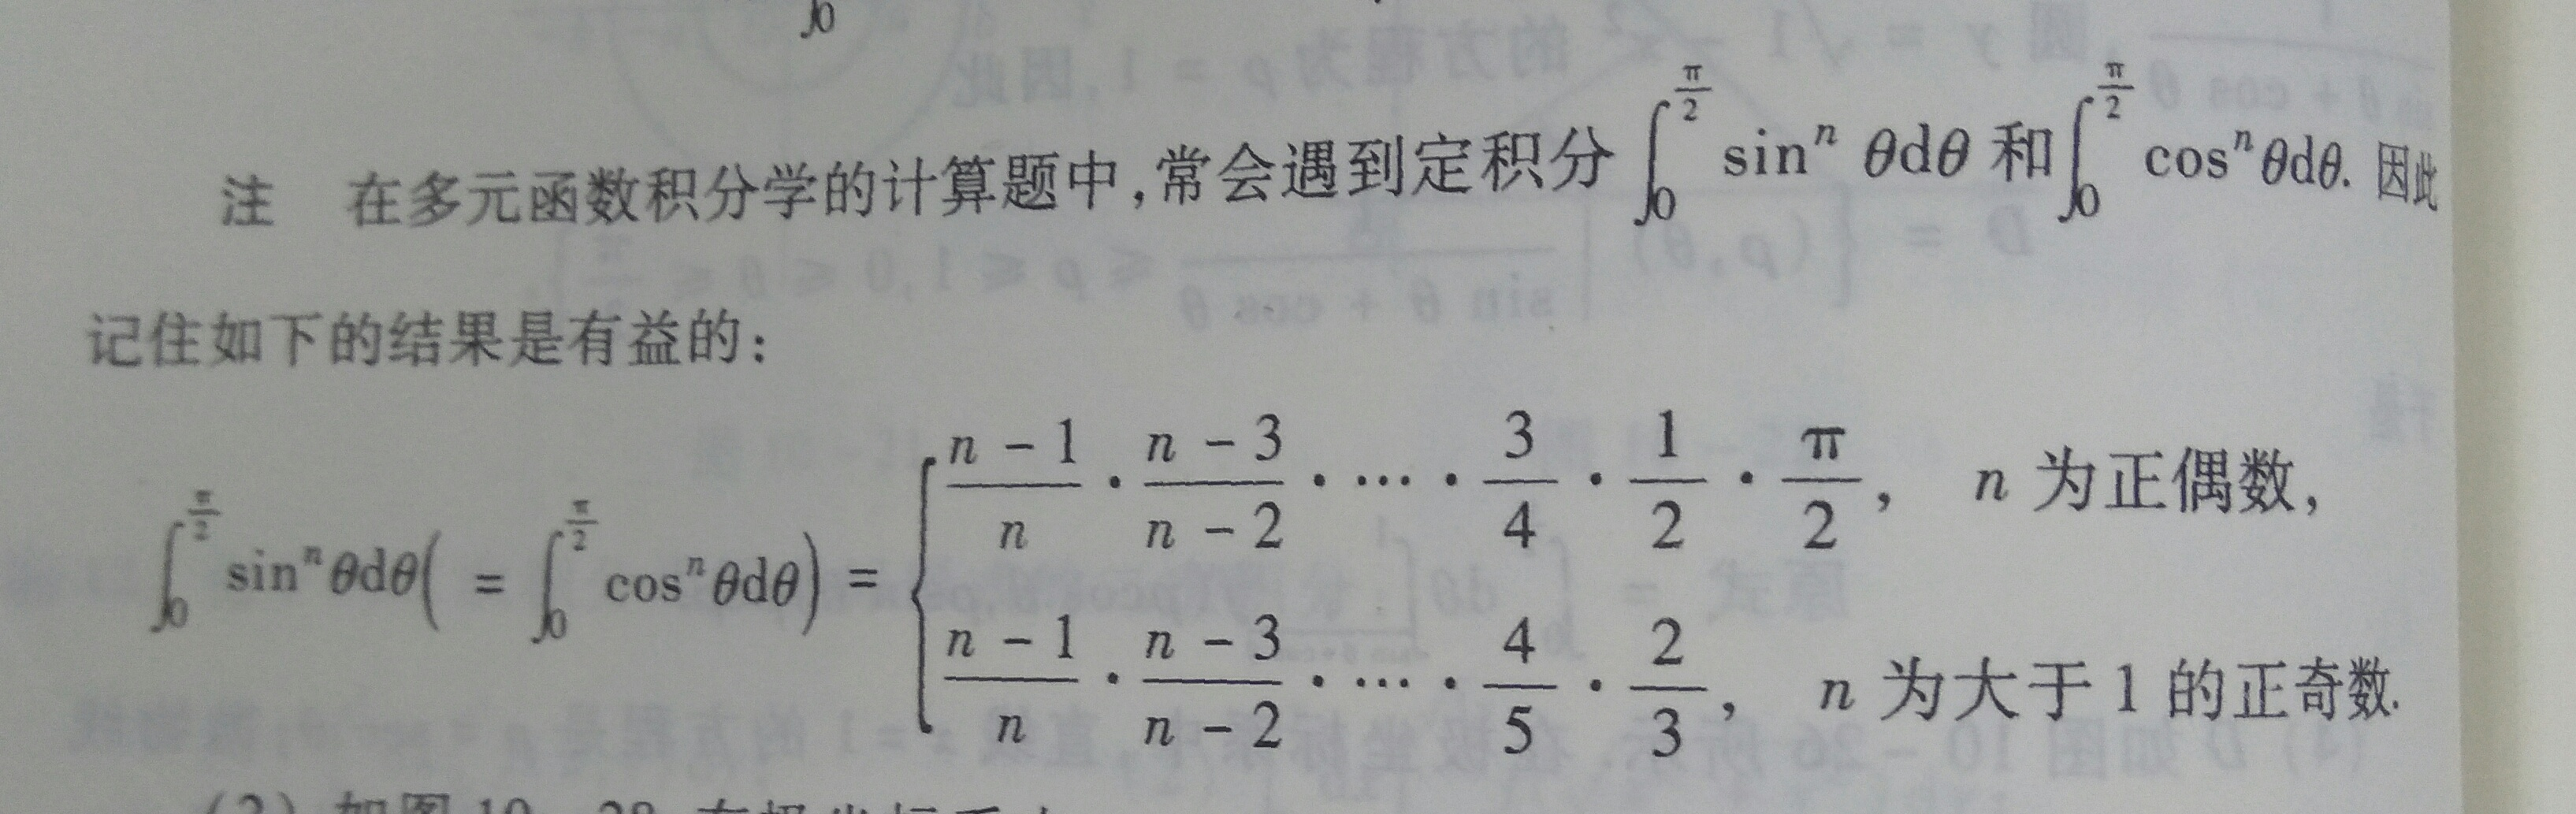
\includegraphics{9345E7/BC4953D356B80A0D6BFD5765D6517251.jpg}
\item
  经典不等式\\
  \[ 2\left| ab \right| \leq a^2+b^2\]
  \[ \left| a \pm b \right| \leq |a|+|b|\]
  \[ \left| |a| - |b| \right| \leq |a-b|\]
  \[\sqrt{ab} \leq \frac{a+b}{2} \leq \sqrt{\frac{a^2+b^2}{2}}\] 当
  x\textgreater{}0,y\textgreater{}0,p\textgreater{}0,q\textgreater{}0,\(\frac{1}{p}+\frac{1}{q}=1 \rightarrow xy \leq \frac{x^p}{p}+\frac{y^q}{q}\)\\
  \[(a^2+b^2)(c^2+d^2) \geq (ac+bd)^2\]\\
  \[ [\int_a^b f(x)g(x)dx]^2 \leq \int_a^b f^2(x)dx\cdot \int_a^b g^2(x)dx\]\\
  \[\mbox{当} p>1, \frac{1}{p}+\frac{1}{q}=1 \mbox{时;} \left| \int_a^b f(x) \cdot g(x)dx\right| \leq \left[ \int_a^b \left| f(x) \right|^p dx \right] ^\frac{1}{p} \cdot \left[ \int_a^b \left| g(x) \right|^q dx \right] ^\frac{1}{q}\]\\
  \[e^x \geq x+1 ; x-1 \geq \ln x ; \frac{1}{1+x} < \ln \left( 1+ \frac{1}{x} \right) < \frac{1}{x}\]
\item
  若\(\int^{(n−1)}(x)\)最多只有一个实零点,则f(x)最多只有n个不同实零点
\item
  \(f^′(x)≠0\) 且连续⇒ f(x)单调\\
\item
  连续的\textbf{奇}函数的\textbf{一 切}原函数都是\textbf{偶}函数
\item
  连续的\textbf{偶}函数的\textbf{仅有一个}原函数都是\textbf{奇}函数\\
\item
  变限积分 存在必连续\\
\item
  可积函数在区间内必有界 (二元也成立)\\
\item
  f(x)是以ㄒ为周期的可积函数\\
  \[ \int_0^\frac{\pi}{4} \sin x dx =1- \frac{\sqrt{2}}{2}\]\\
  \[ \int_\frac{\pi}{4}^\frac{\pi}{2} \sin x dx =\frac{\sqrt{2}}{2}\]\\
  \[ \int_0^\frac{\pi}{2} \sin x dx = 1\]\\
  \[ \int_0^\pi \sin x dx =2\]\\
\item
  积分递归解法\\
  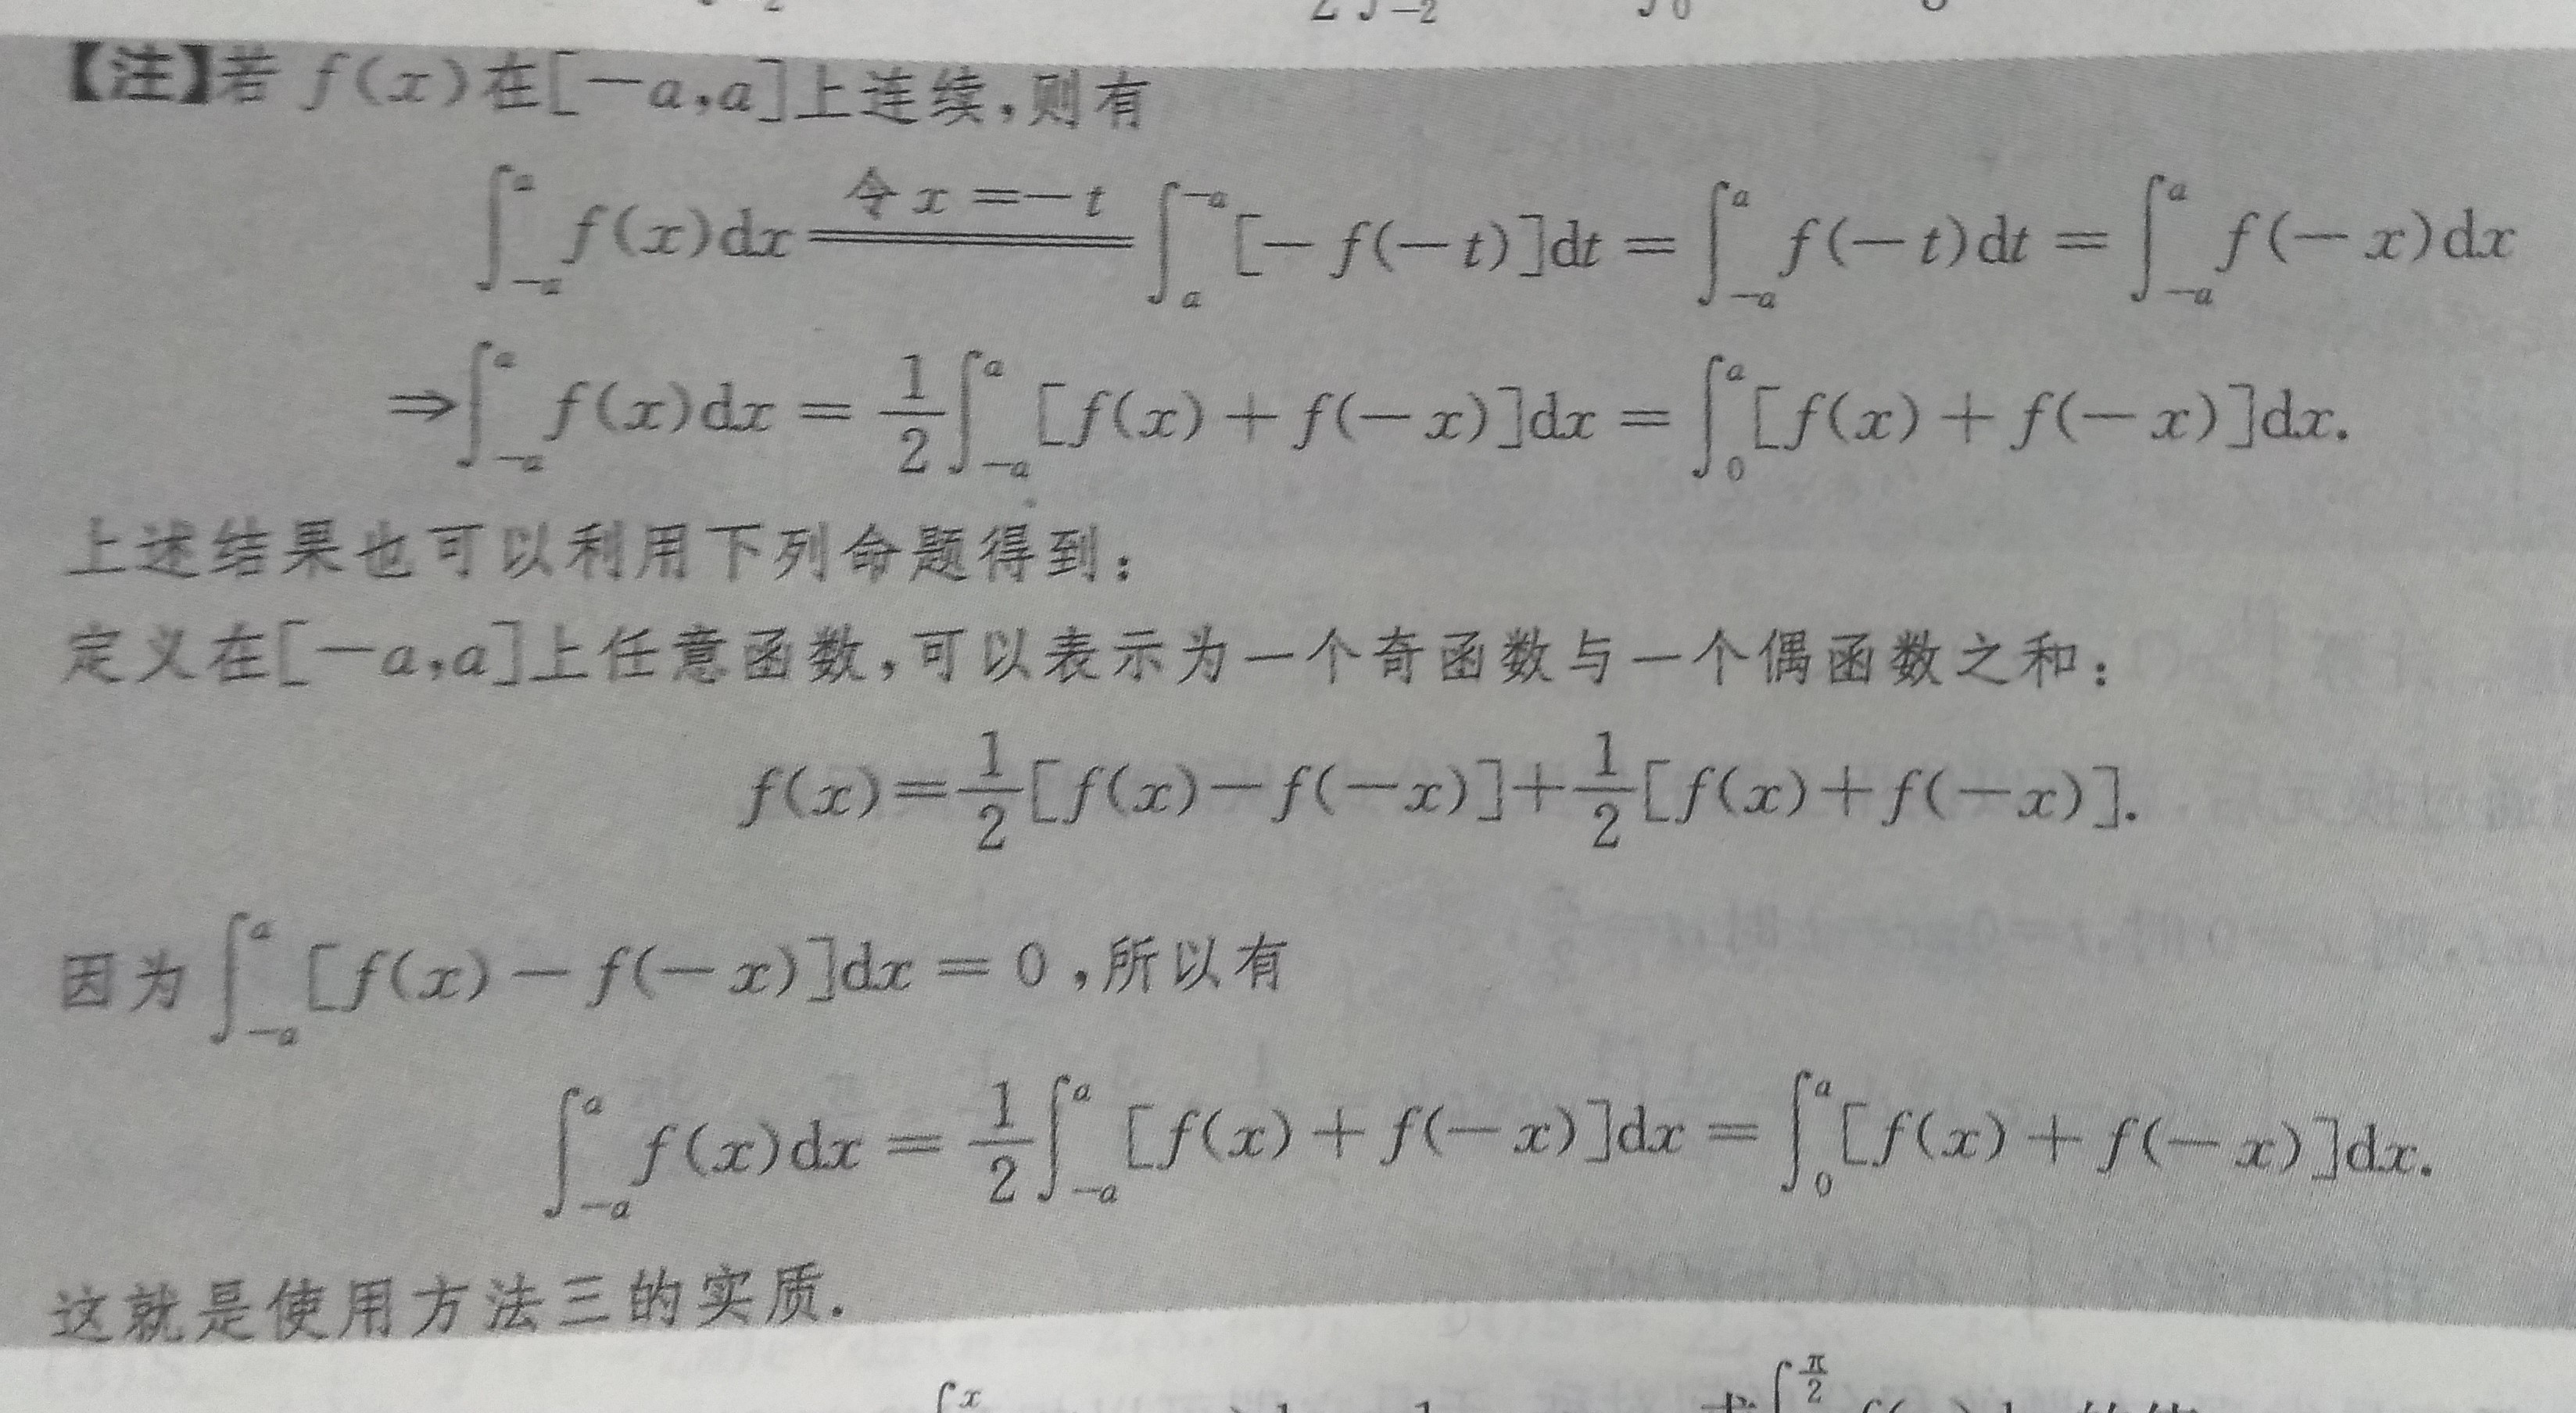
\includegraphics{9345E7/2002379869.jpg}
\end{enumerate}

    \begin{enumerate}
\def\labelenumi{\arabic{enumi}.}
\tightlist
\item
  极值判定充分条件

  \begin{enumerate}
  \def\labelenumii{\arabic{enumii}.}
  \tightlist
  \item
    f '(x\textsubscript{0})左右异号→极值点\\
    \$ \left\{

    \begin{aligned}
    &f'=0 \\
    &f''(x_0) \neq 0
    \end{aligned}

    \right. \rightarrow \mbox{极值点} \$\\
  \item
    当\$ f\^{}\{(n)\} (x\_0) \neq 0\$

    \begin{enumerate}
    \def\labelenumiii{\arabic{enumiii}.}
    \tightlist
    \item
      n为偶\\
      \$f\^{}\{(n)\} (x\_0) \leq 0 \$ → 极大值\\
      \$f\^{}\{(n)\} (x\_0) \geq 0 \$ → 极小值\\
    \item
      n为奇\\
      拐点\\
    \end{enumerate}
  \end{enumerate}
\item
  多元函数极值与最值\\
  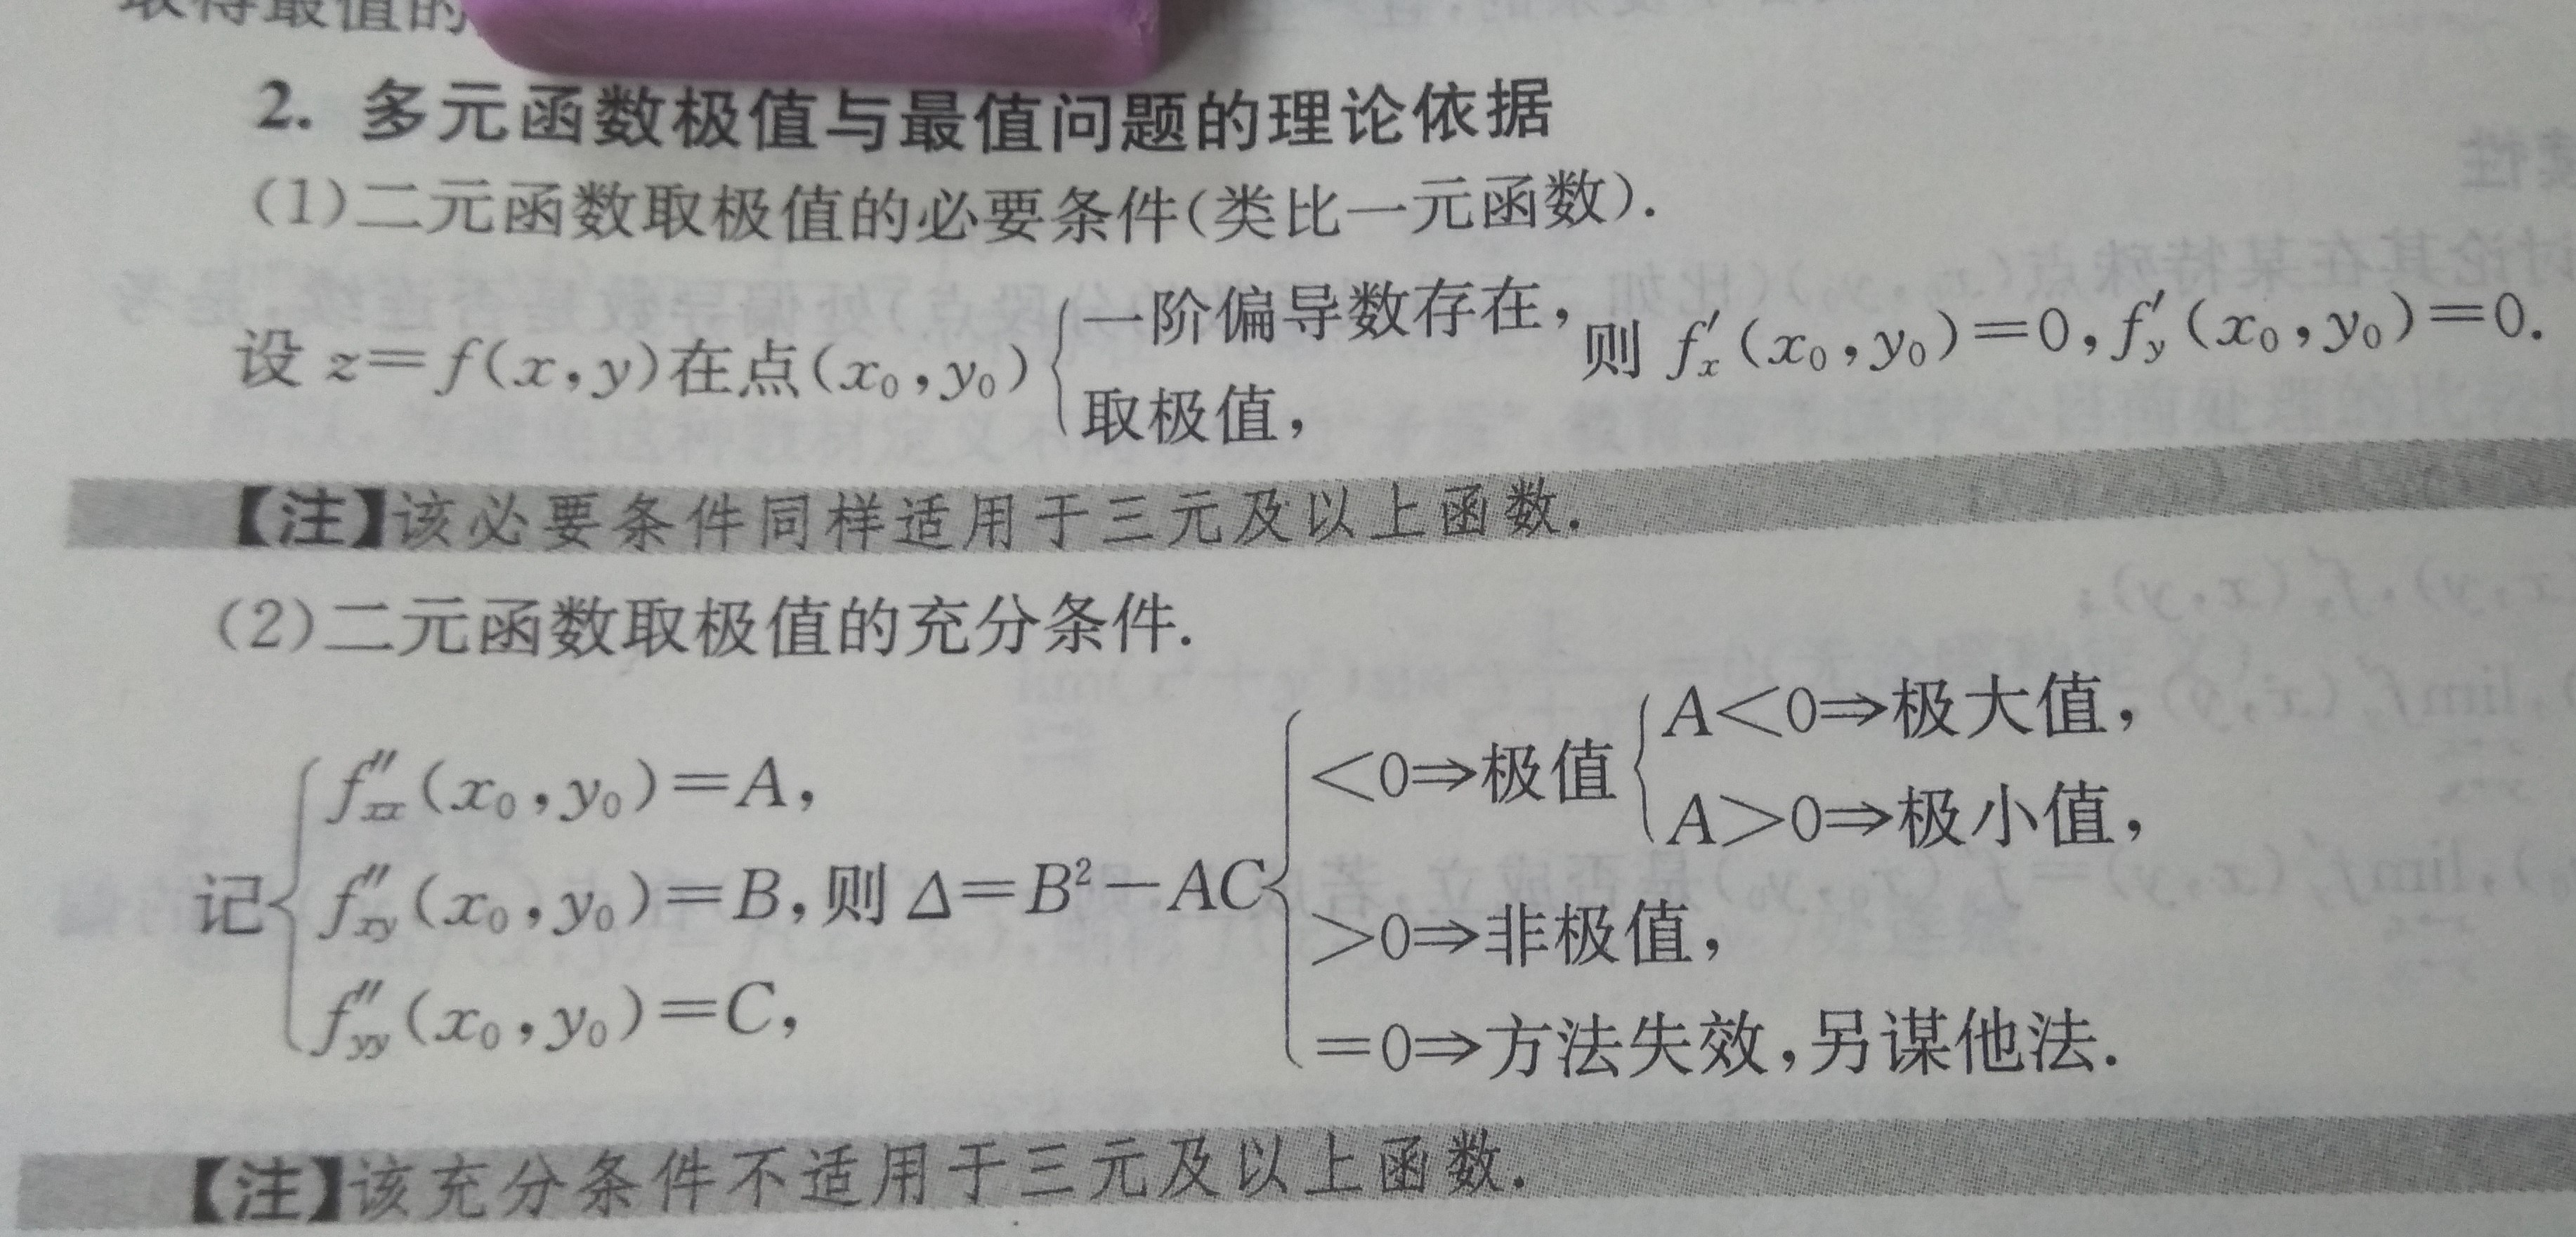
\includegraphics{9345E7/2805530637.jpg}\\
\item
  凹凸性定义

  \begin{enumerate}
  \def\labelenumii{\arabic{enumii}.}
  \tightlist
  \item
    凹 \$ f(\frac{x_1+x_2}{2}) \textless{} \frac{f(x_1)+f(x_2)}{2}\$\\
  \item
    凹 \$ f{[}λx\_1 +(1-λ)x\_2{]} \leq λf(x\_1)+(1-λ)f(x\_2)\$\\
  \end{enumerate}
\item
  极值点与拐点不要求导数存在\\
  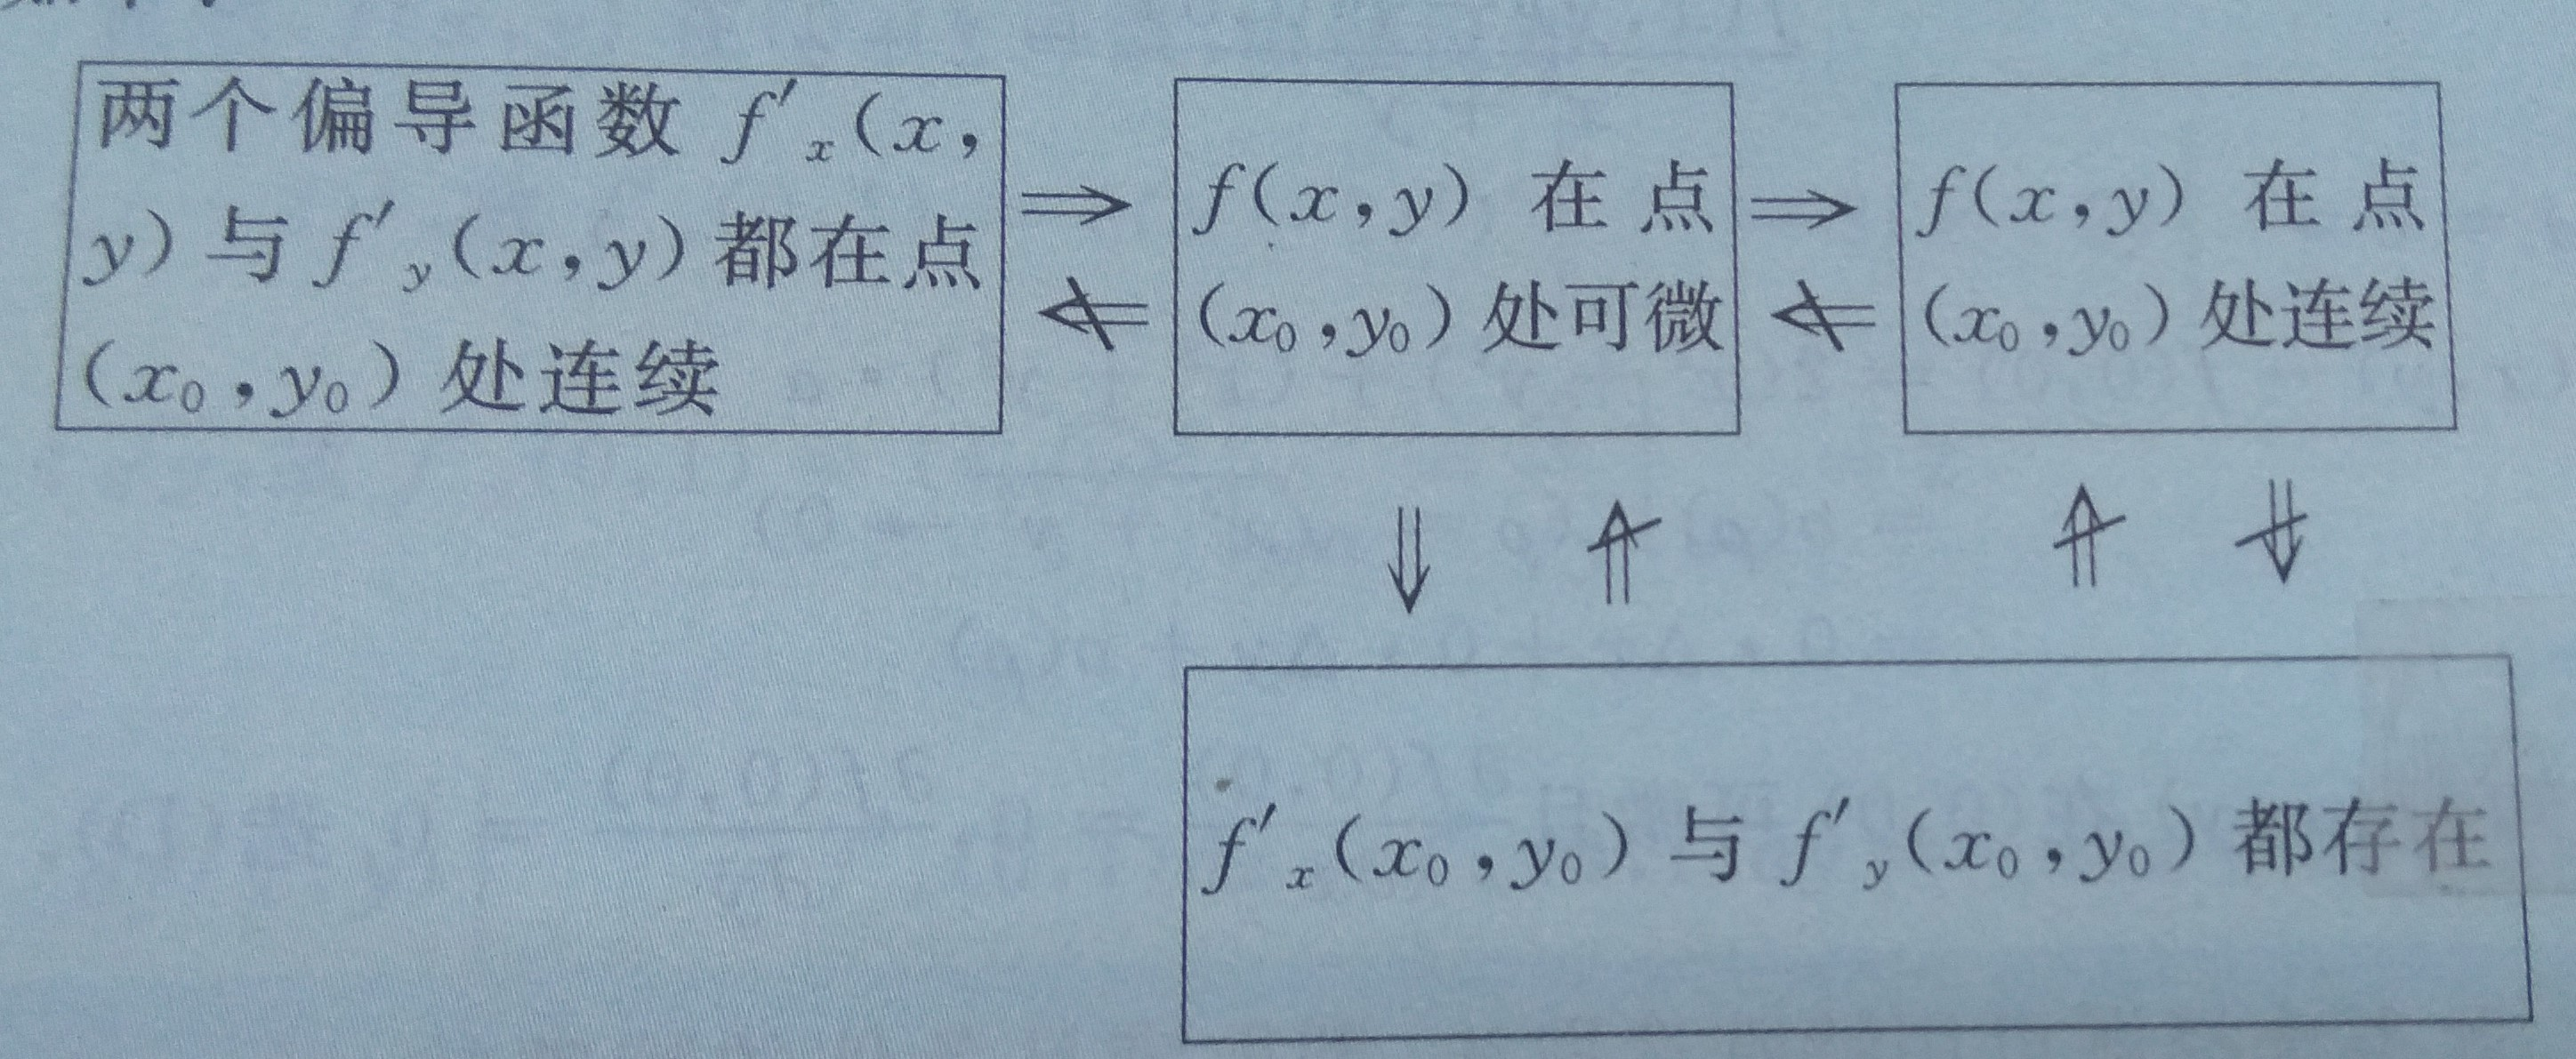
\includegraphics{9345E7/2367085874.jpg}\\
\item
  曲率半径\\
  \$ k= \frac{|y''|}{{(1+y'^2)}^{3 \over 2}}\$\\
  R= \$ \frac{1}{k}=\frac{{(1+y'^2)}^{3 \over 2}}{|y''|}\$\\
\item
  弧长L=\$ \int\_α\^{}β \sqrt{r^2(θ)+[r'(θ)]^2}dθ\$\\
\item
  曲边扇形面积 S=\$ \frac{1}{2}
  \int\_α\textsuperscript{β\textbar{}r\_1}2(θ)-r\_2\^{}2(θ)\textbar{}dθ\$\\
\item
  极座标交换积分次续\\
  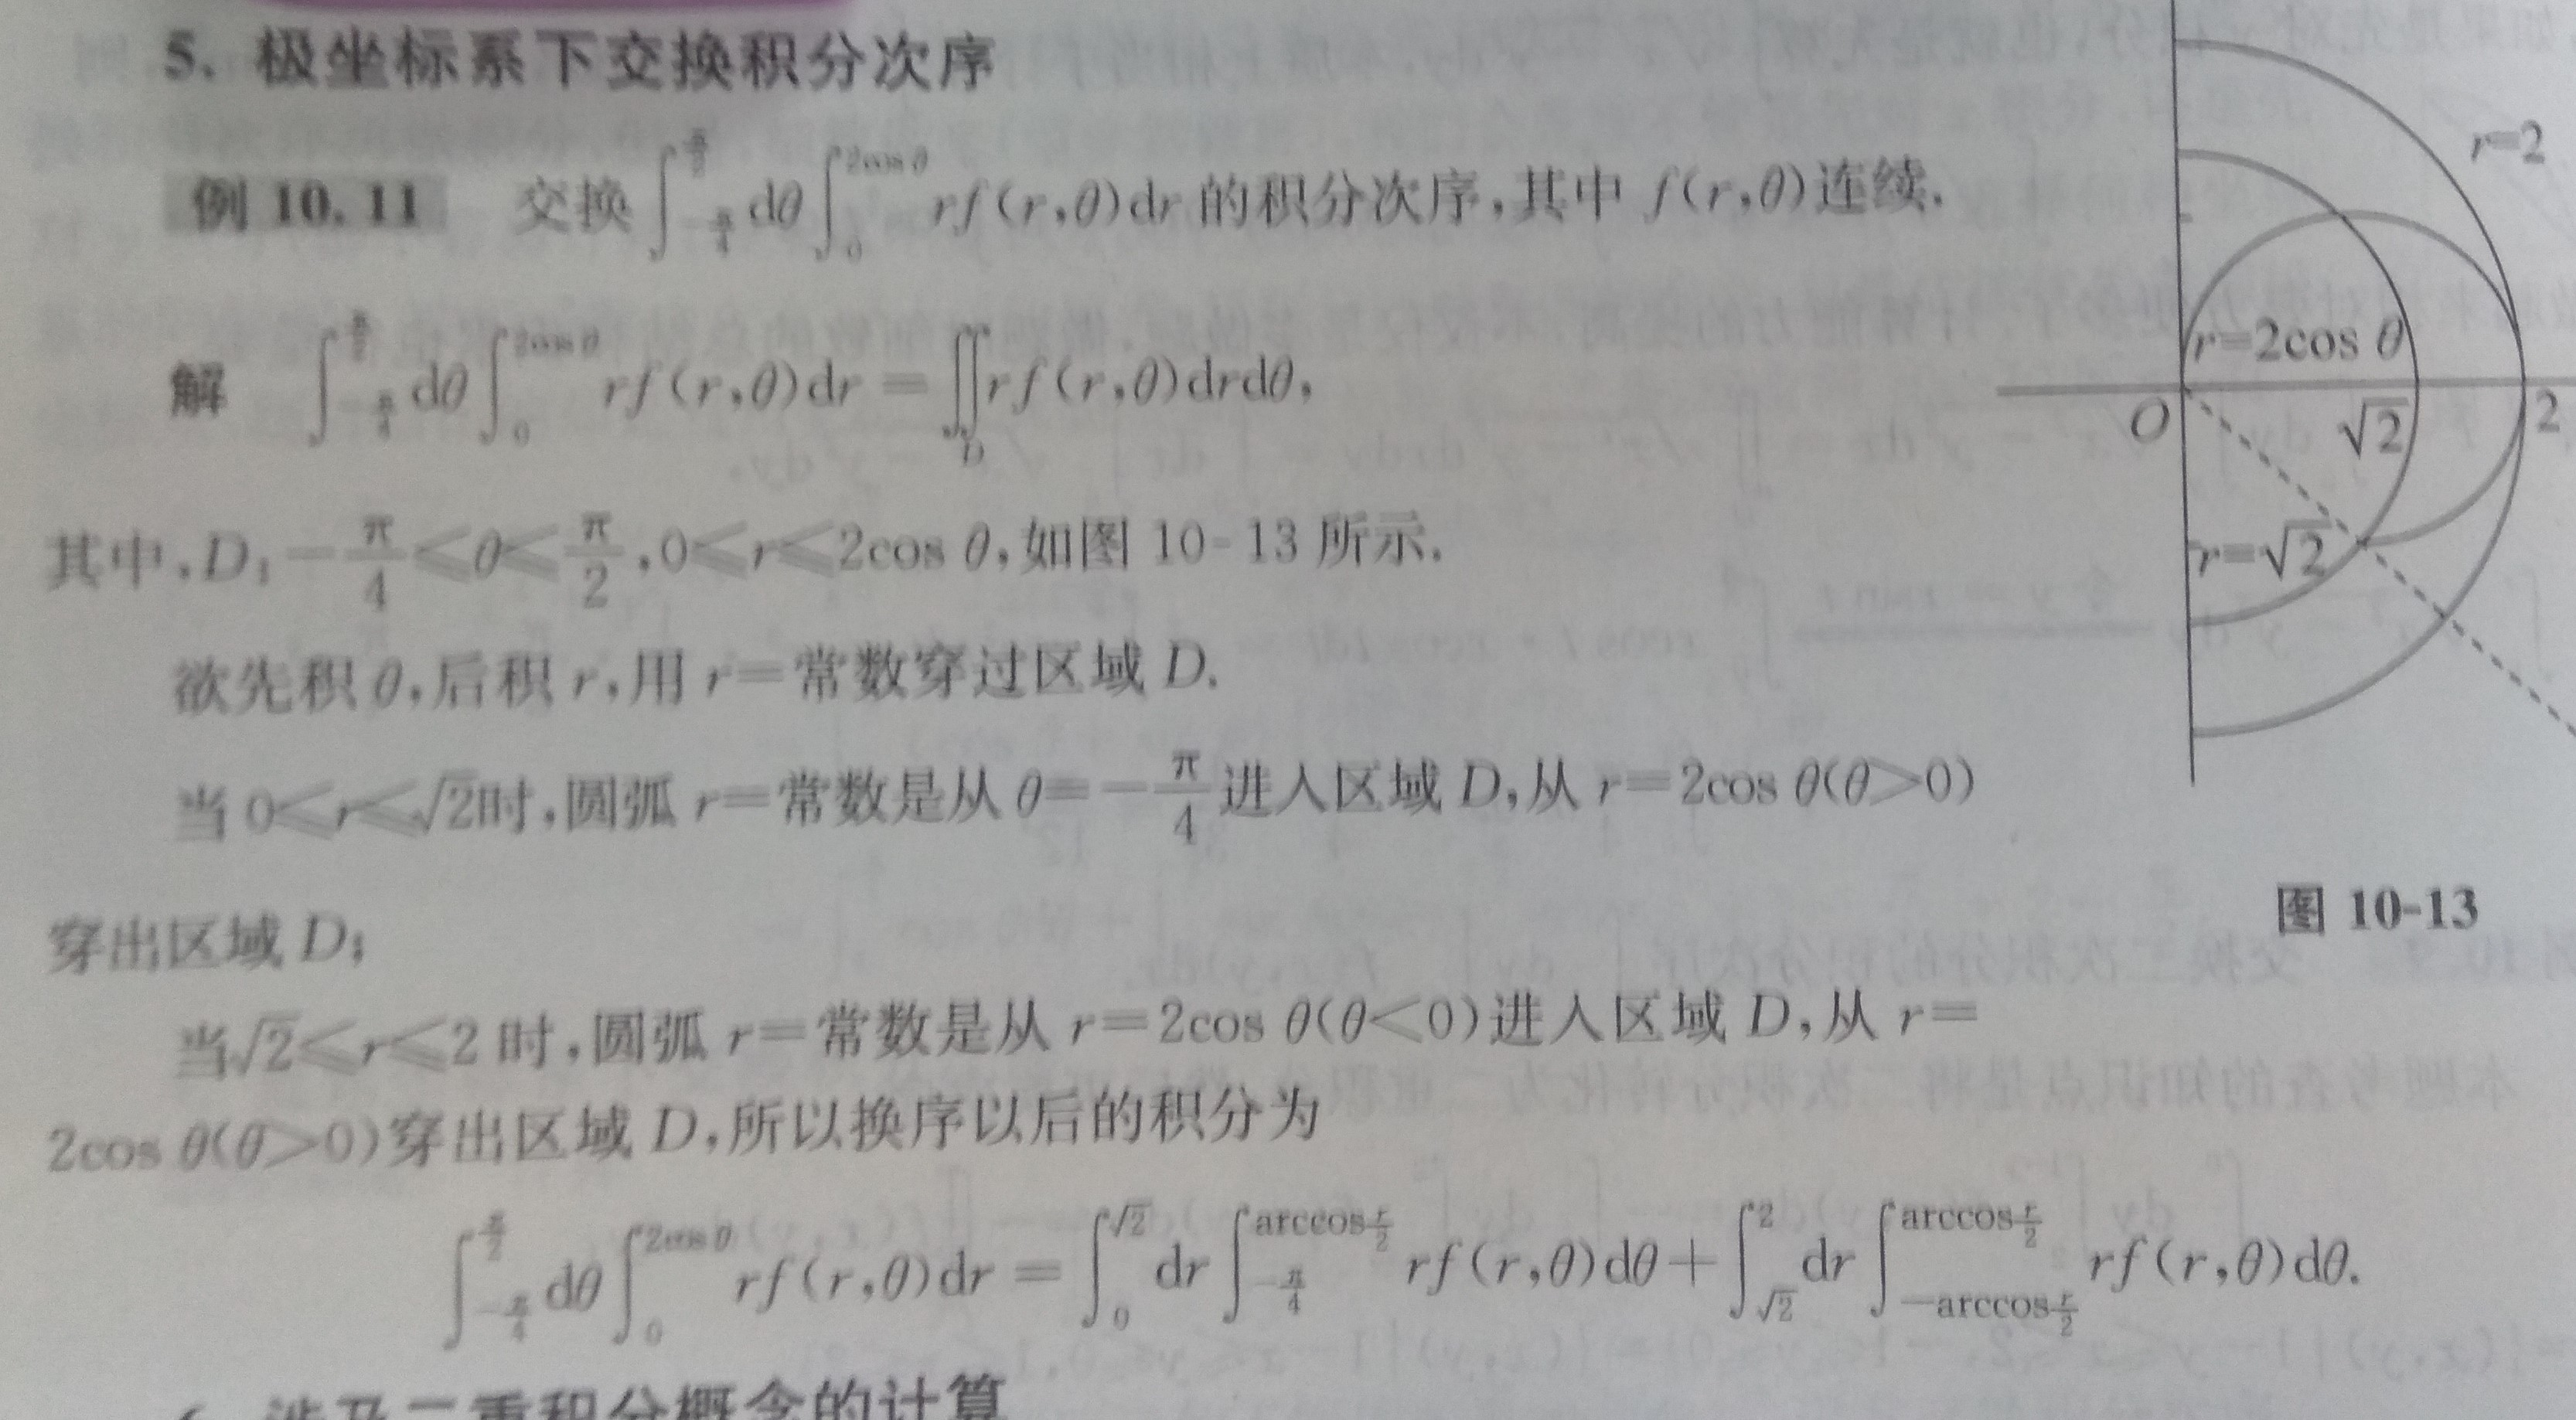
\includegraphics{9345E7/3720754172.jpg}\\
\item
  反常积分审敛\\
  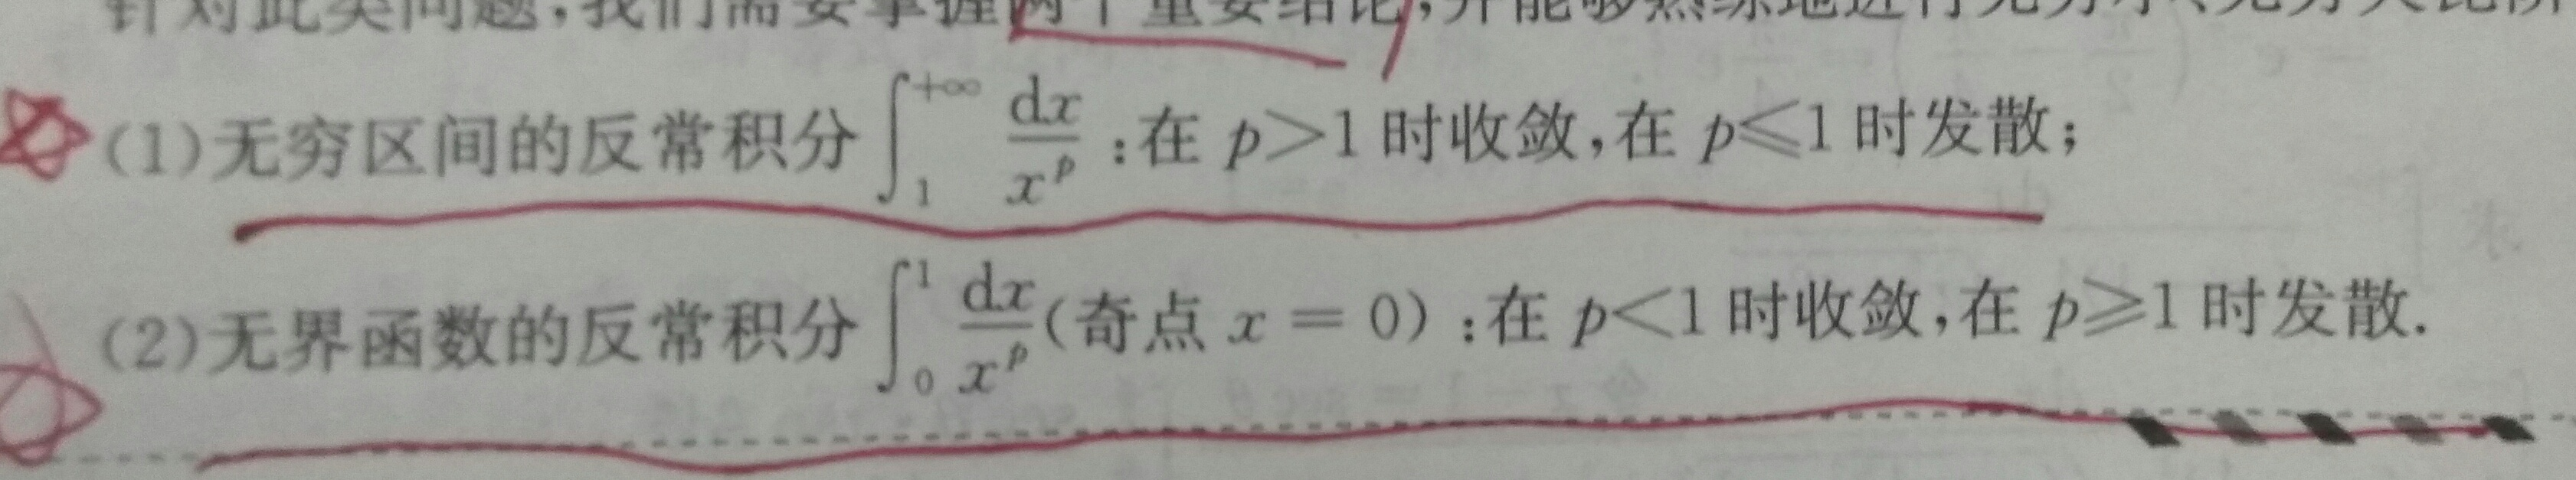
\includegraphics{9345E7/2059466188.jpg}
\item
  一阶微分方程 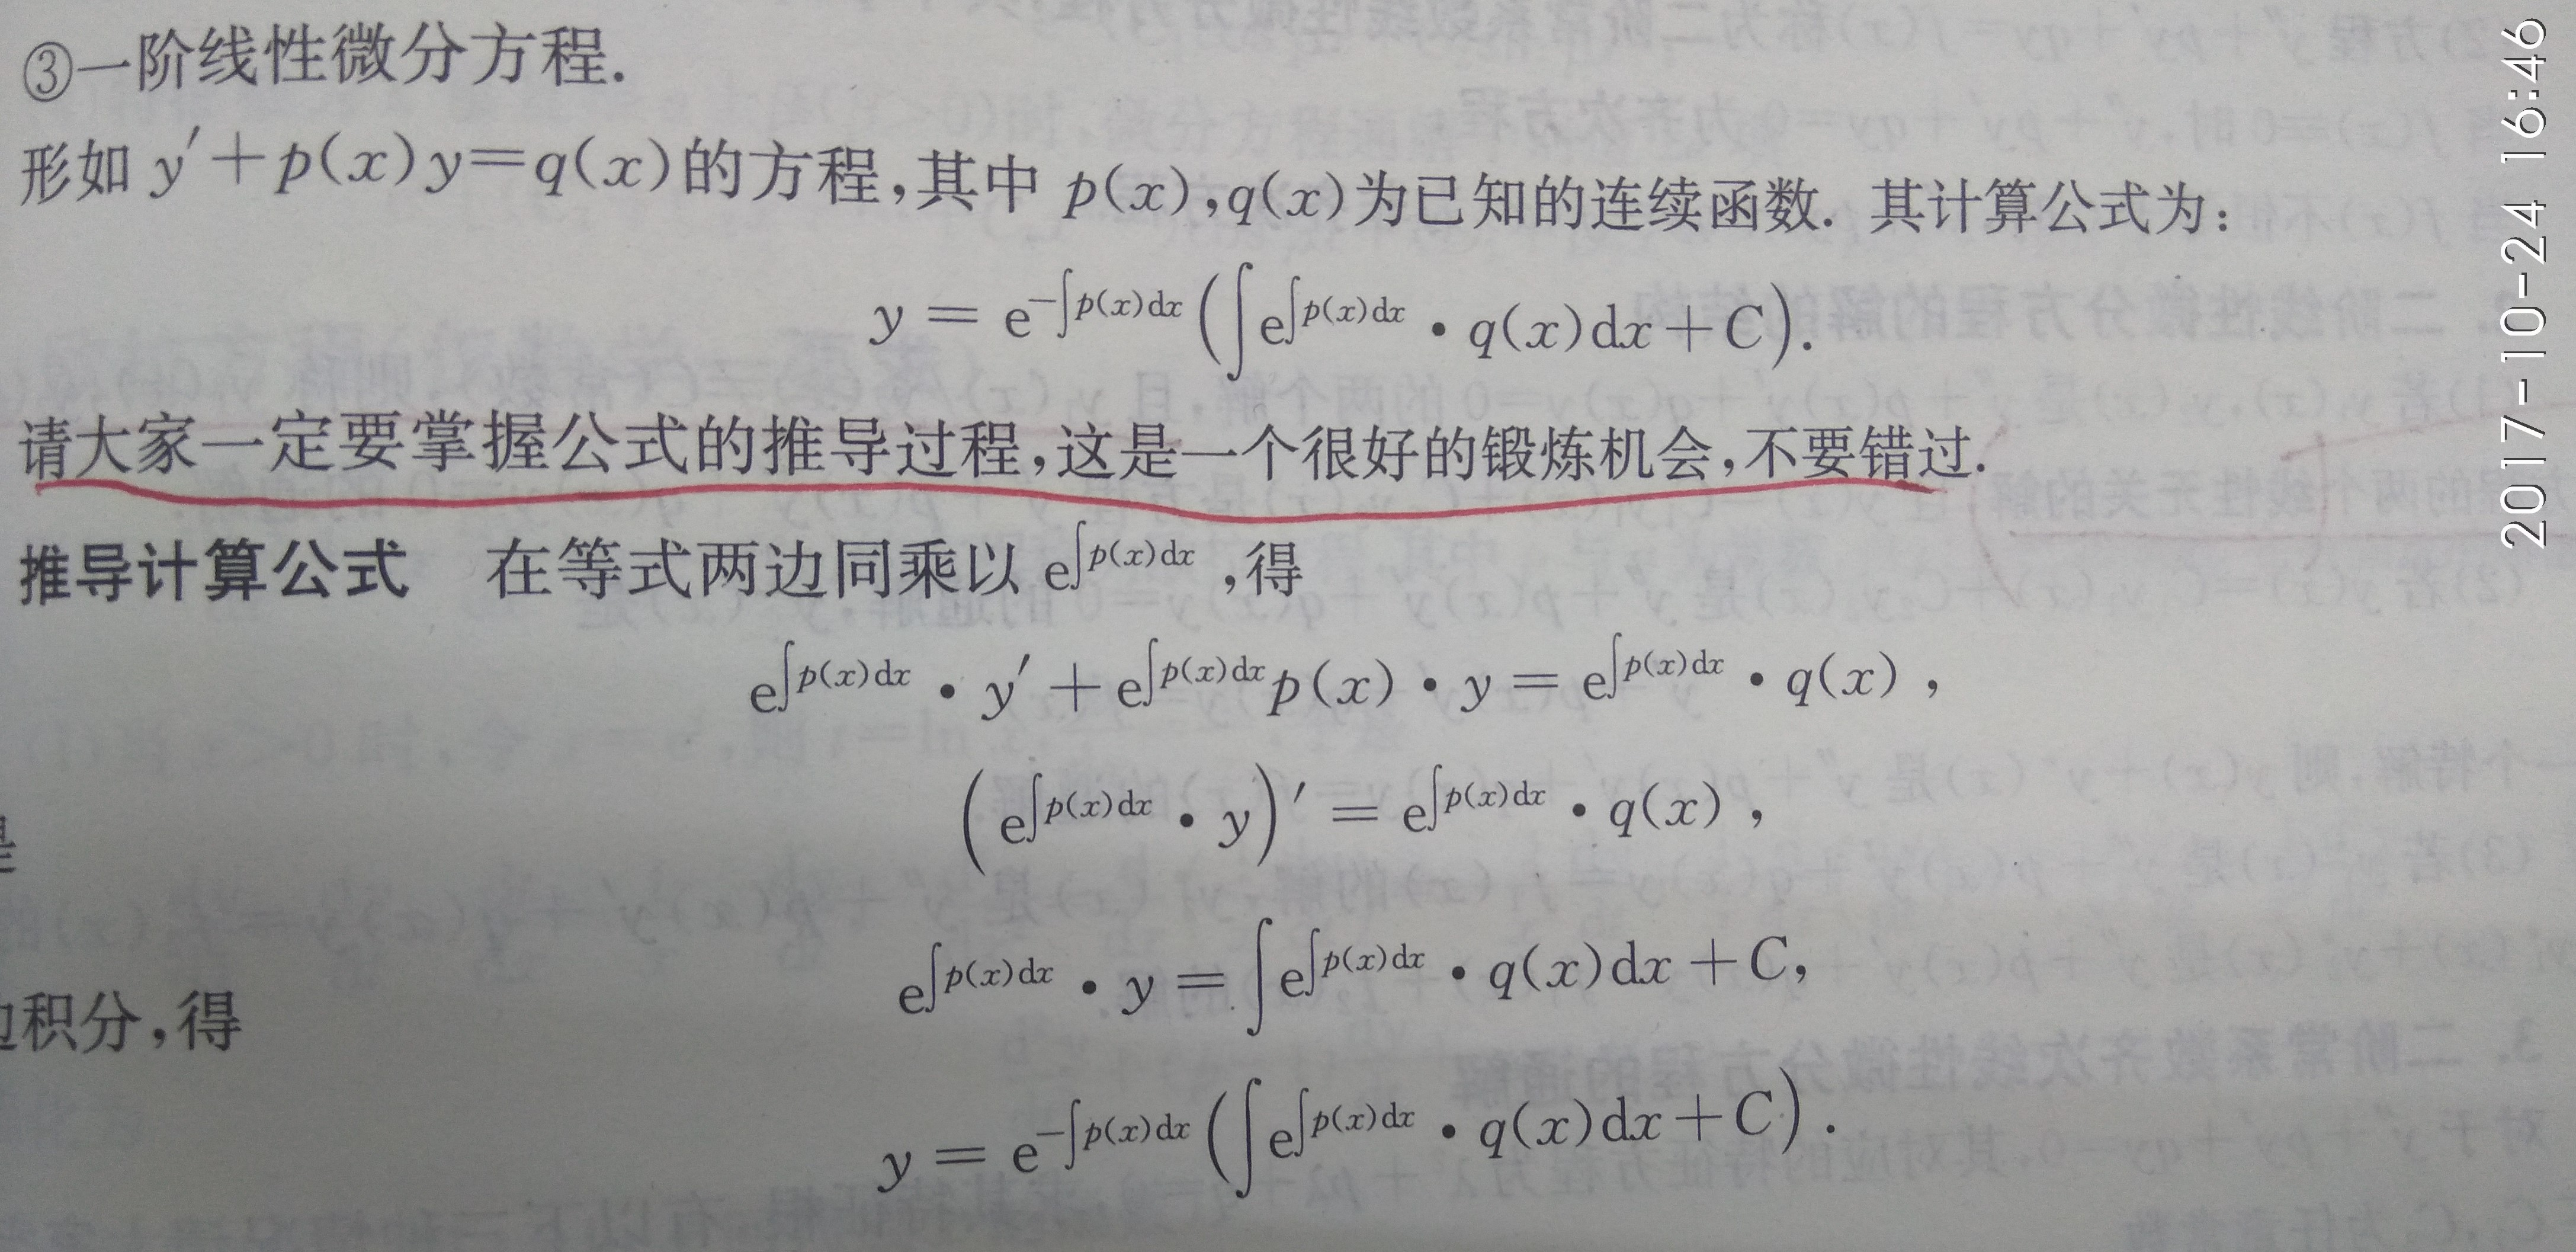
\includegraphics{9345E7/677562795.jpg}\\
\item
  一阶微分方程\\
  当 \$ u=\frac{y}{x} ⇉ y=ux\frac{dy}{dx}=u+x\frac{du}{dx}\$\\
  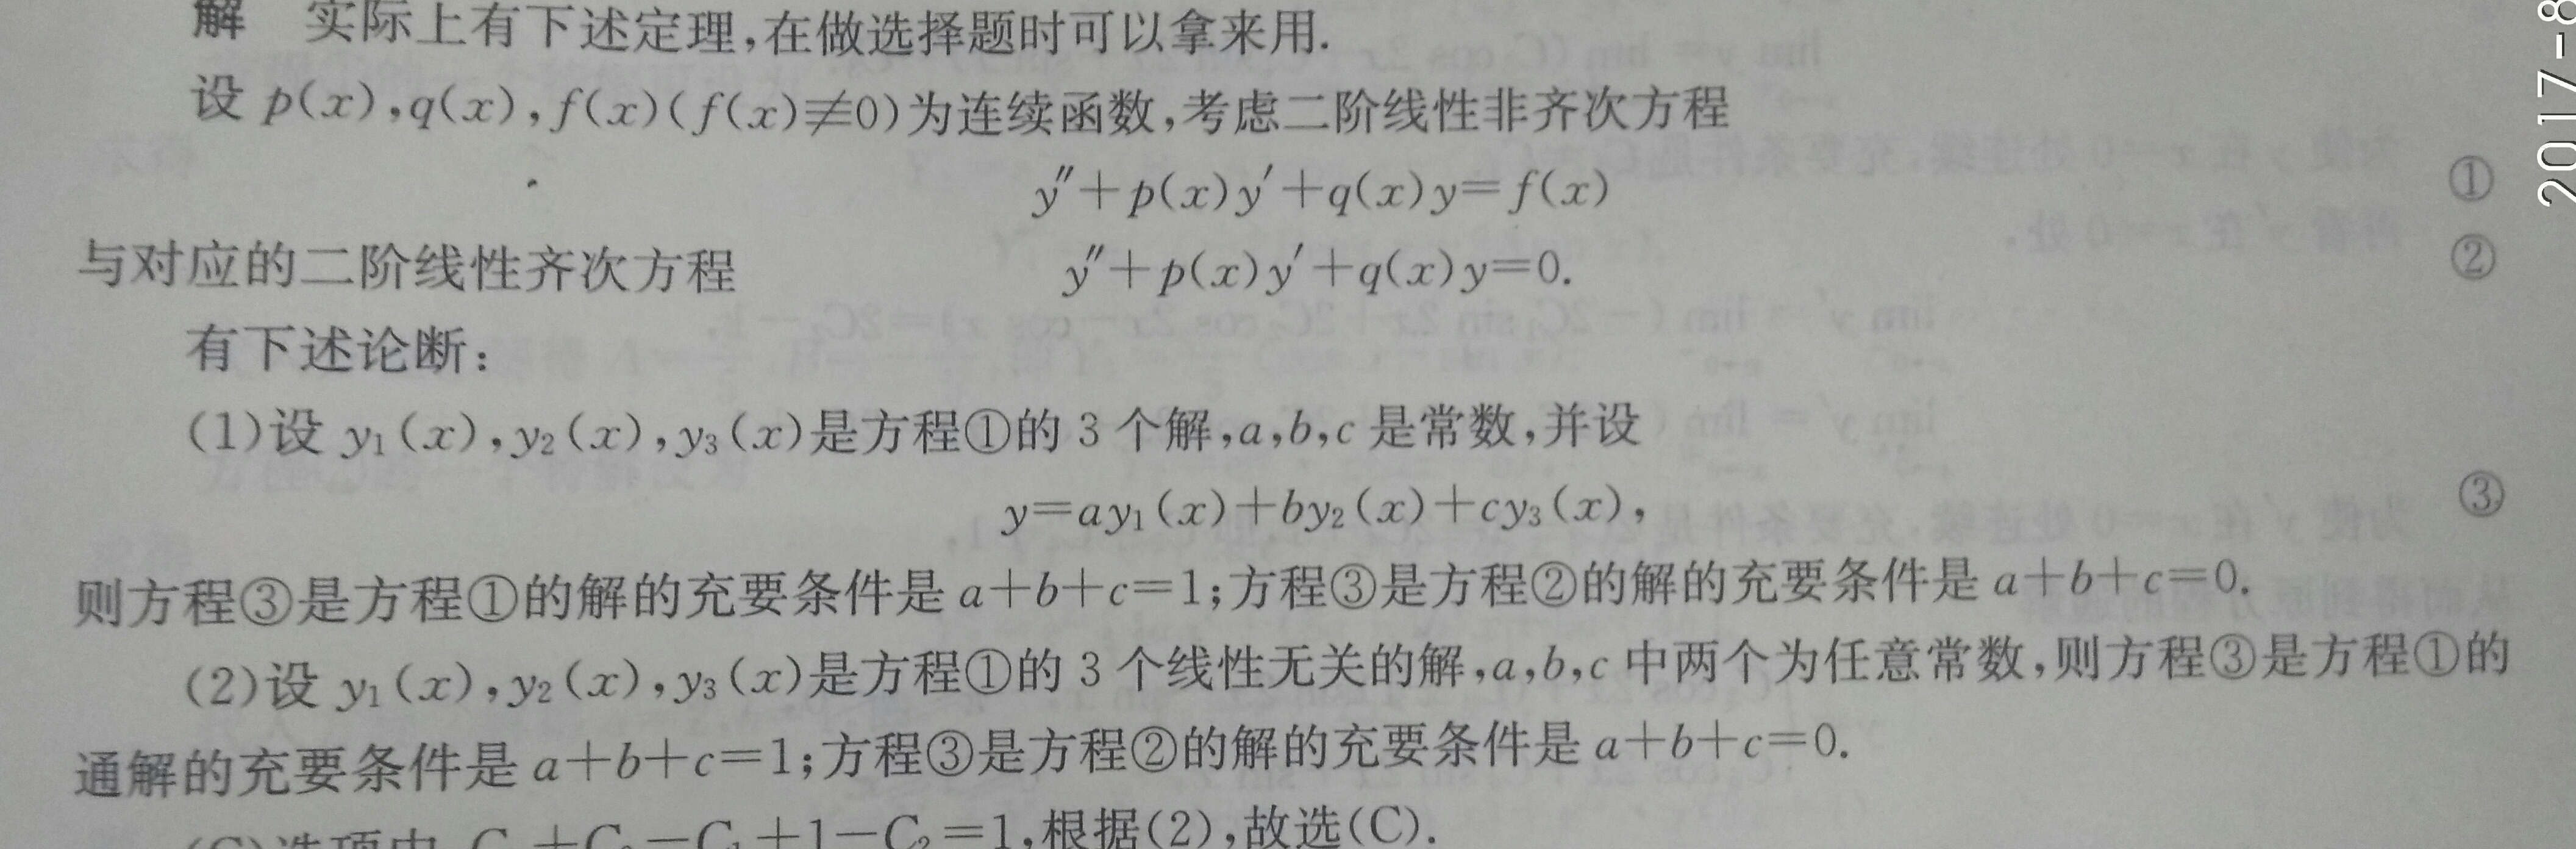
\includegraphics{9345E7/478763472.jpg}\\
  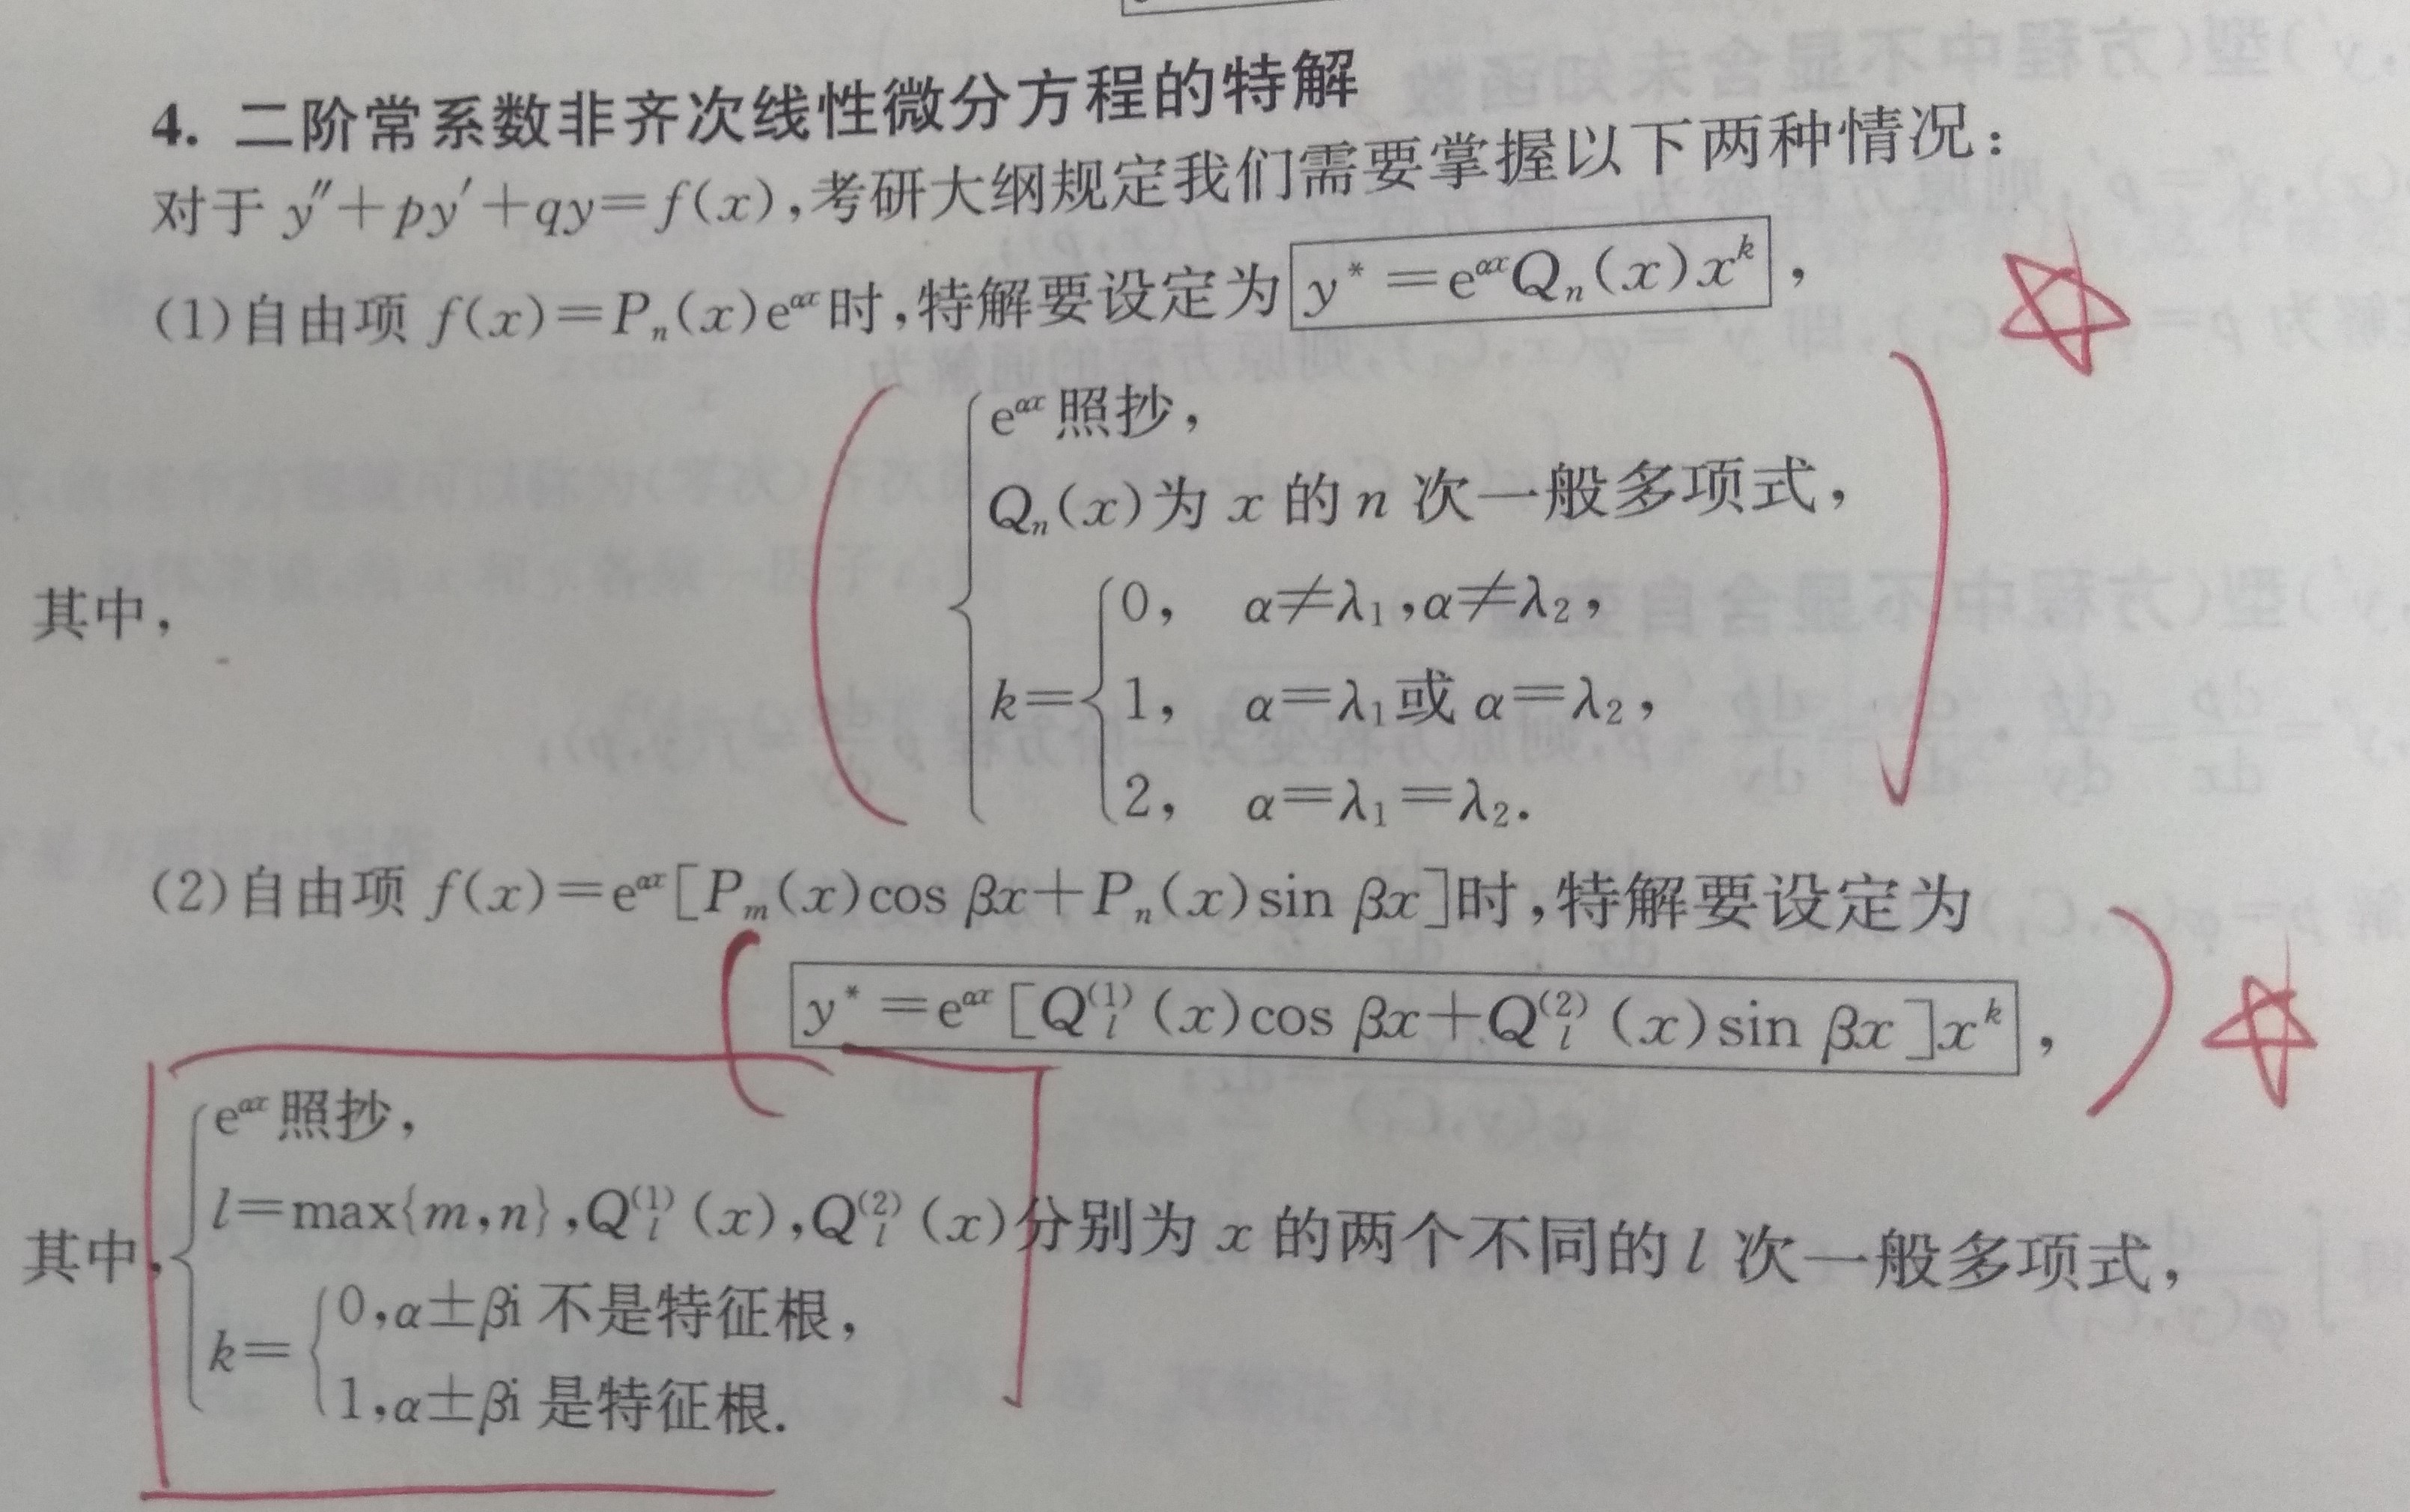
\includegraphics{9345E7/595734581.jpg}\\
  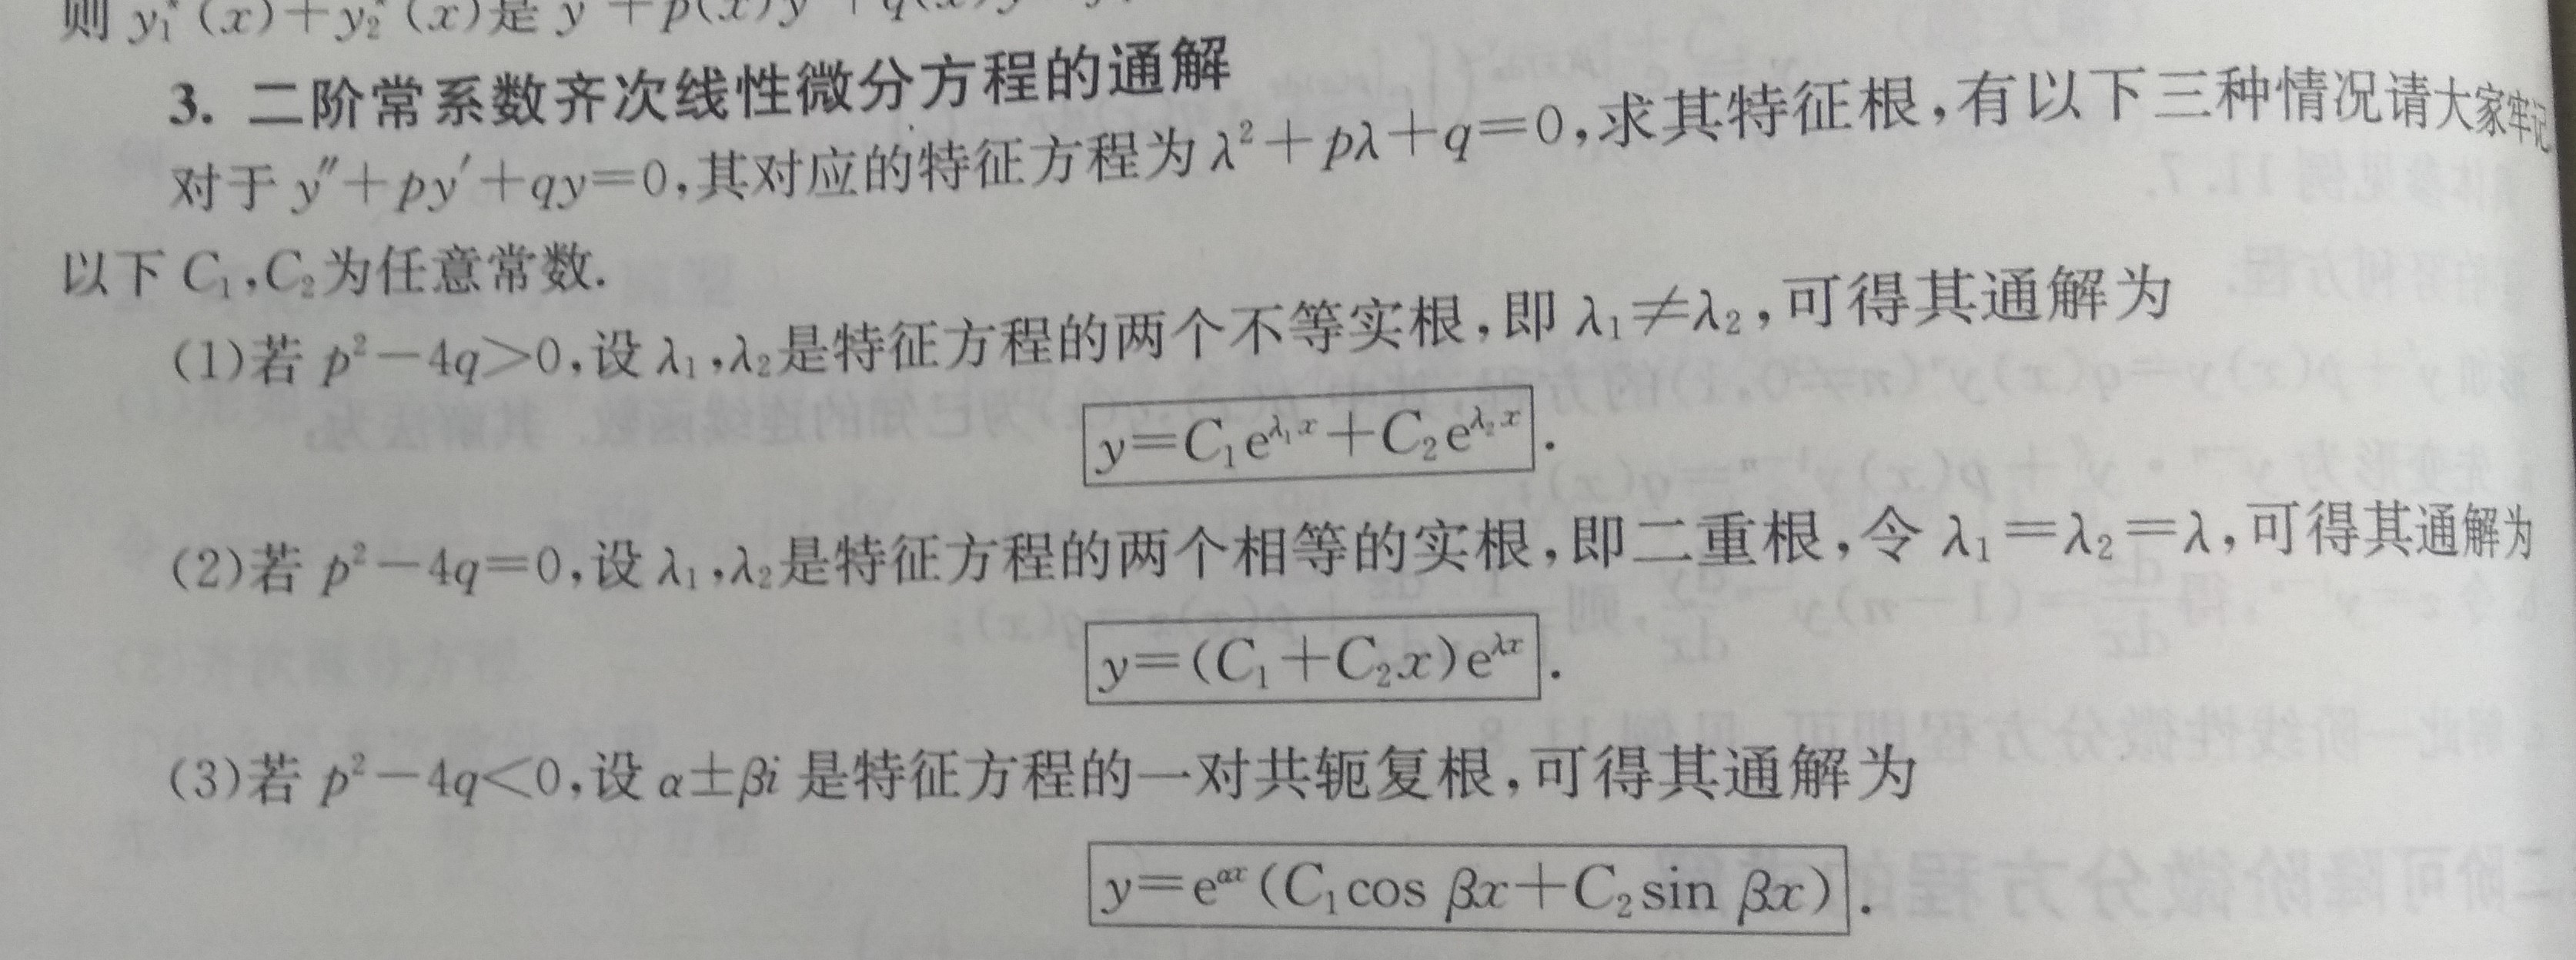
\includegraphics{9345E7/601054614.jpg}
\end{enumerate}

    隐藏 {[}comment{]}: \textless{}\textgreater{} (This is a comment, it
will not be included) {[}comment{]}: \textless{}\textgreater{} (in the
output file unless you use it in) {[}comment{]}:
\textless{}\textgreater{} (a reference style link.) {[}//{]}:
\textless{}\textgreater{} (This is also a comment.) {[}//{]}: \# (This
may be the most platform independent comment)


    % Add a bibliography block to the postdoc
    
    
    
    \end{document}
